\chapter{Risultati Sperimentali}\label{ch:esperimenti}
Il capitolo illustra e discute i risultati sperimentali ottenuti applicando i modelli proposti su task relativi a dataset reali.

Il paragrafo~\ref{sec:esperiment:dataset} descrive i dataset utilizzati ed i corrispondenti task affrontati.

Il paragrafo~\ref{sec:esperiment:esperimenti} descrive i setting sperimentali e raccoglie i risultati ottenuti.

Il paragrafo~\ref{sec:esperiment:considerazioni} espone un'analisi critica dei risultati sperimentali.


%%%%%%%%%%%%%%%%%%%%%%%%%%%%%%%%%%%%%%%%%%%%%%%%%%%%%%%%%%%%%%%%%%%%
\section{Dataset}\label{sec:esperiment:dataset}
Le potenzialità dei modelli proposti sono state sperimentate su problemi reali appartenenti all'ambito della Chimica. 

Pur senza addentrarsi nei dettagli è interessante sottolineare come il legame fra il Machine Learning e la Chimica vada recentemente rafforzandosi, in particolar modo in relazione all'apprendimento di dati su domini strutturati. L'enorme varietà di molecole naturalmente rappresentabili come grafi, i costi sperimentali elevati, l'esistenza di conoscenze non sempre codificabili o prone a numerose eccezioni, fanno infatti della Chimica il banco di prova ideale per dei modelli in grado di gestire domini strutturati.

\`E dunque alla sfera della Chemioinformatica che vanno ascritti i task affrontati ed i dataset che verranno descritti nel seguito del paragrafo.

Prima di procedere, è importante sottolineare che nessuna specifica conoscenza pregressa è stata necessaria per preprocessare i dati, modificarne la struttura o estrapolarne informazioni numeriche. In altri termini, le informazioni utilizzate per allenare i modelli sono esattamente quelle riportate nei dataset: diversamente da quanto accade ricorrendo ad altri approcci, nessuna particolare assunzione riguardante il dominio trattato è stata fatta (e.g.\ la scelta di una metrica nell'uso di un kernel) né è stata praticata alcuna forma di feature-selection manuale (e.g.\ la selezione di indici topologici).

\subsubsection*{Predictive Toxicology Challenge}\label{sec:esperimenti:dataset:ptc}
Il \emph{Predictive Toxicology Challenge} (PTC) \cite{Helma:ThePTC} ha fornito i dati per quattro task distinti. Il dataset consta di $417$ molecole in formato \emph{Structure Data Format} (SDF) di cui è riporta la carcinogenicità riferita a diversi tipi di roditori: topi maschi (MM), topi femmine (FM), ratti maschi (MR), ratti femmine (FR). 

Ogni molecola è stata rappresentata come un grafo indiretto, con i vertici corrispondenti agli atomi e gli archi ai legami atomici. Il grado massimo riscontrato sull'intero dataset è $k = 4$. Il numero di vertici nei grafi in input risulta mediamente $25.7$, variando da un minimo di $2$ ad un massimo di $109$.

L'etichetta numerica associata ad ogni vertice è stata ottenuta codificando il simbolo atomico corrispondente tramite un encoding binario $1$-of-$m$ e concatenando due valori aggiuntivi presenti nel dataset, CHG e RAD, rispettivamente corrispondenti alla carica atomica ed il radical dell'atomo. La dimensione totale delle etichette di input è dunque $24$. 
La figura~\ref{fig:molecole} mostra l'esempio due molecole appartenenti al dataset PTC, rappresentate come grafi indiretti, e schematizza il processo di encoding del simbolo atomico.
\begin{figure}[tbp]
\centering
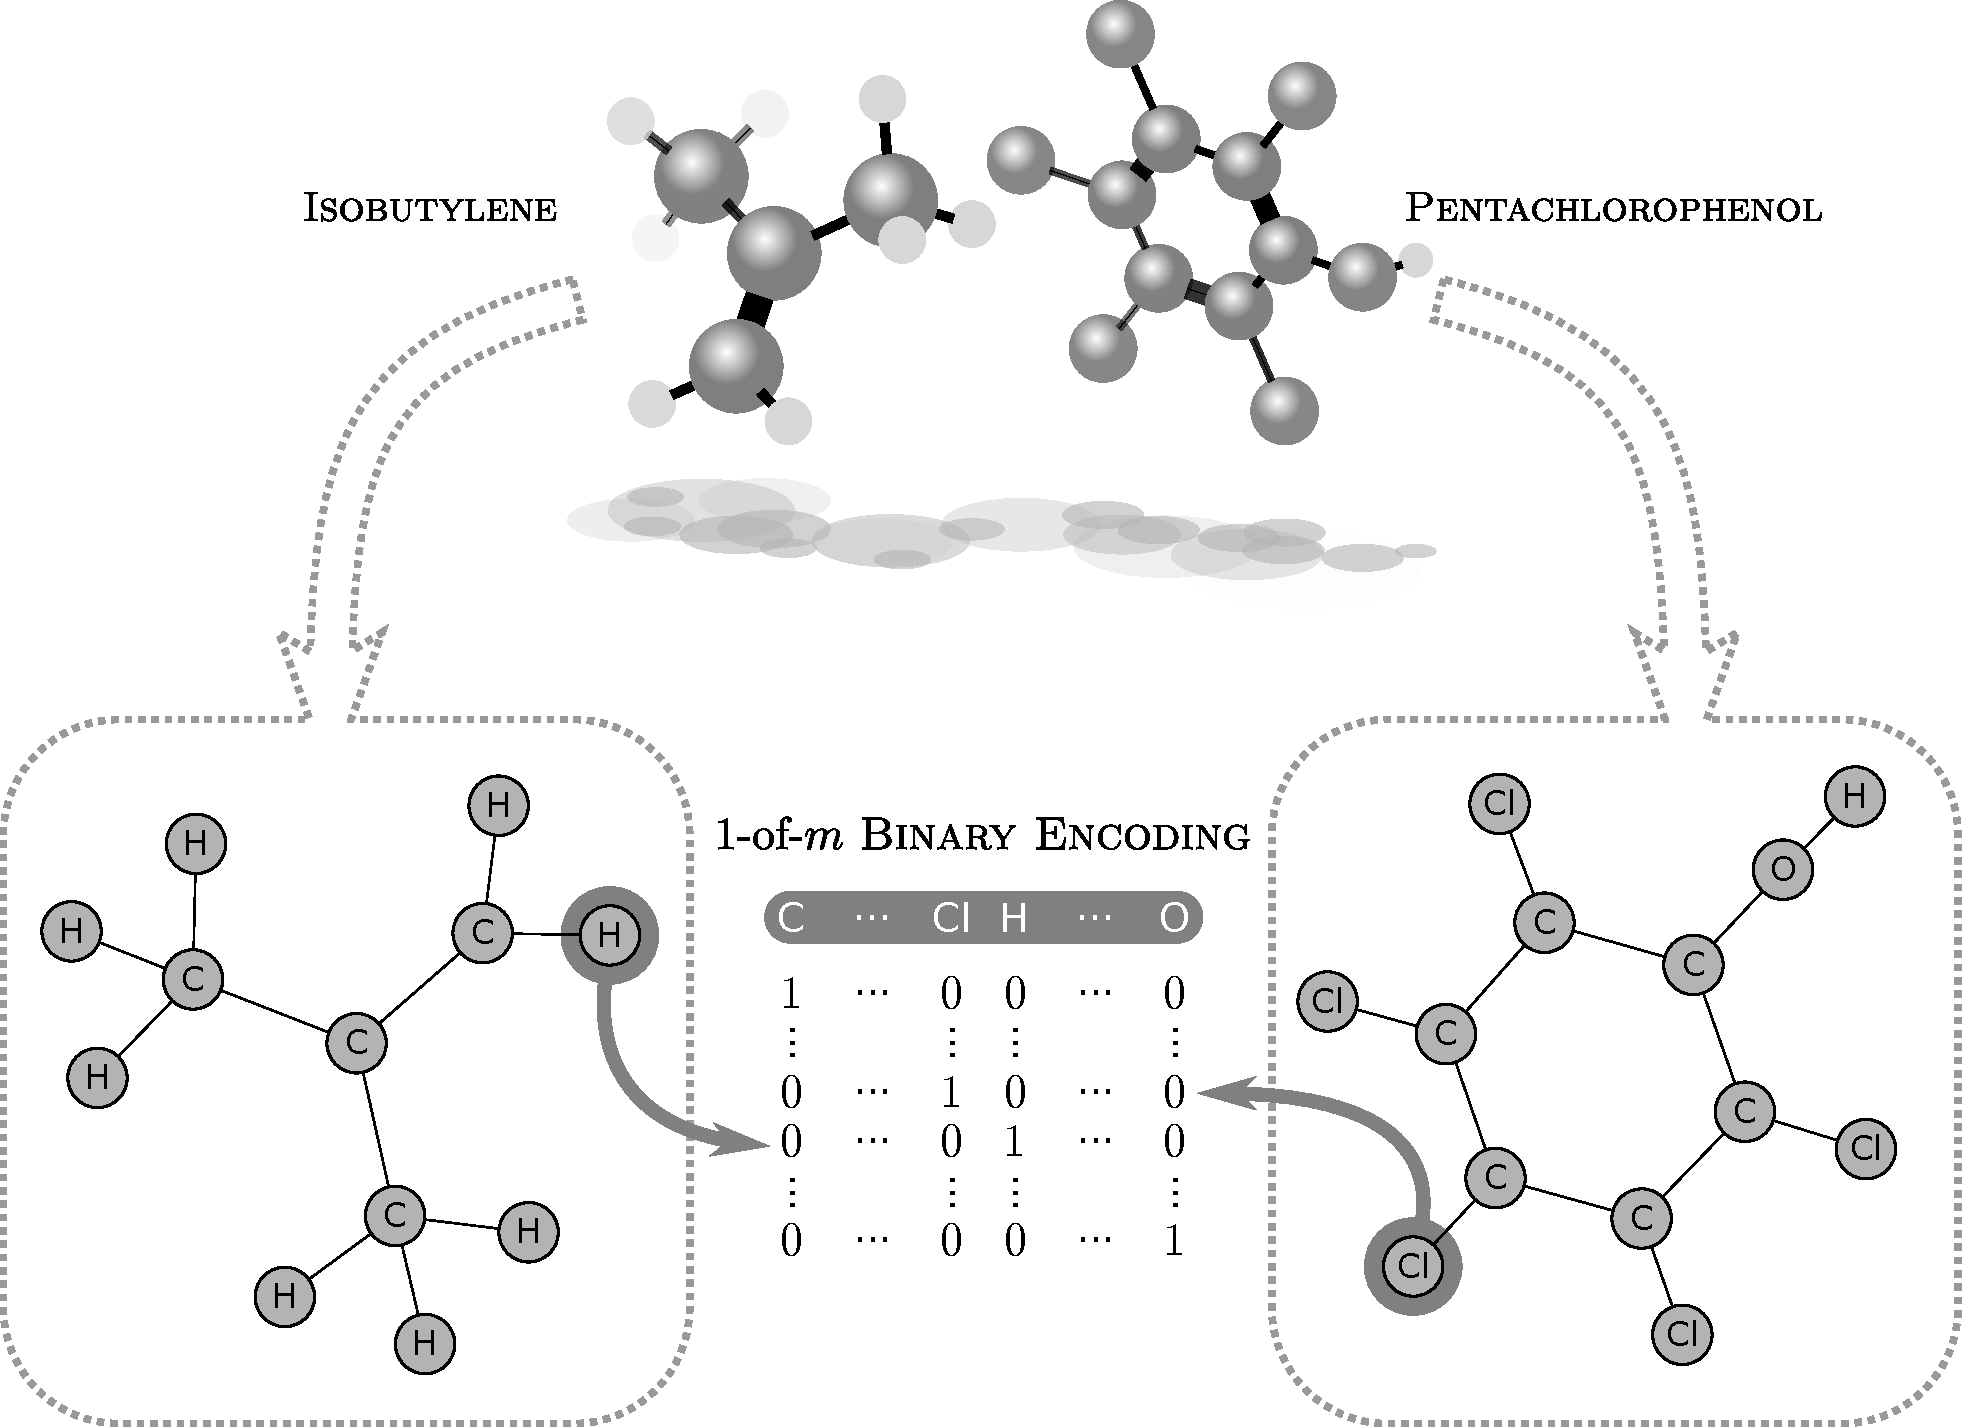
\includegraphics[width=0.9\columnwidth]{img/molecole-v2}
\medskip
\caption[Rappresentazione dell'input]{Rappresentazione dell'input in forma di grafo ed encoding del simbolo atomico.}
\label{fig:molecole}
\end{figure}

Quattro task structure-to-element di classificazione binaria sono stati definiti per PTC, uno per ogni tipo di roditore \cite{Frohlich:OptimalAssignment}, assegnando target $+1$ alle molecole attive e target $-1$ a quelle inattive.

\subsubsection*{Mutagenesis}\label{sec:esperimenti:dataset:mutag}
La seconda serie di task affrontati si riferisce al dataset \emph{Mutagenesis} \cite{Srinivasan:Mutagenesis} (Mutag), contenente 230 molecole nitroaromatiche in formato Progol\footnote{\url{http://www.doc.ic.ac.uk/~shm/progol.html}}, di cui è indicata la mutagenicità.
Ogni composto nel dataset è descritto dalla sua struttura atomo-legame (AB), da due valori corrispondenti a misurazioni di proprietà chimiche della molecola (C) e due attributi strutturali precalcolati (PS). Riprendendo quanto fatto in \cite{Gallicchio:GraphESN}, sono state dunque considerate le tre possibili descrizioni: AB, AB+C, AB+C+PS.

Ogni molecola del dataset è stata rappresentata come un grafo indiretto, con vertici ed archi corrispondenti ad atomi e legami rispettivamente, entrambi riportati nella descrizione AB dei singoli composti. Il grado massimo riscontrato sul dataset risulta essere $k = 4$. Il numero di vertici per input varia tra un minimo di $13$ ad un massimo di $40$, con una media di $25.6$ vertici per ogni molecola.

L'etichetta numerica associata ad ogni vertice dell'input è stata ricavata codificando il simbolo atomico corrispondente attraverso un encoding binario $1$-of-$m$ e poi concatenando la carica parziale dell'atomo, il tipo atomico normalizzato in $[-1,1]$ più gli altri valori globali contenuti nella descrizione C e PS, in accordo alla rappresentazione via via adottata. La dimensione delle etichette di input è dunque di 11, 13 e 15 per le descrizioni AB, AB+C e AB+C+PS rispettivamente.

Il task sul dataset è stato definito come una classificazione binaria, con il target a $+1$ per i grafi corrispondenti a composti mutageni e $-1$ altrimenti.



\subsubsection*{Bursi}\label{sec:esperimenti:dataset:bursi}
Il dataset \emph{Bursi} \cite{Kazius:Bursi,Ferrari:AnOpenSource} contiene 4204 molecole in formato SDF, di cui è riportata la mutagenicità. Ne risulta un task structure-to-element di classificazione binaria.
Il dataset risulta all'origine suddiviso partizionato in un training-set, contenente 3367 molecole, ed un test-set con 837 composti.

Anche in questo caso le molecole sono state rappresentate come grafi indiretti, con vertici ed archi corrispondenti ad atomi e legami rispettivamente. Nell'input il numero di vertici varia tra un minimo di $4$ ed un massimo di $417$, con una media di $30.3$ vertici per molecola.

L'etichetta numerica associata ai vertici è realizzata attraverso l'encoding binario $1$-of-$m$ del simbolo atomico. Le etichette hanno dunque dimensione $14$. Il grado massimo riscontato sul dataset è $k = 4$.

Il target per il task di classificazione binaria è stato realizzato assegnando valore $+1$ alle molecole attive e $-1$ alle molecole non attive.


\subsubsection*{Angiotensin Converting Enzyme}\label{sec:esperimenti:dataset:ace}
Il dataset \emph{Angiotensin Converting Enzyme} (ACE) \cite{Sutherland:AComparisonOfMethods} contiene 114 ACE-inibitori in formato SDF a cui è associato un valore reale che ne indica l'attività (i.e.\ $\text{plC}_{50}$) in un intervallo che varia tra $2.1$ a $9.9$. Il dataset definisce dunque un task structure-to-element di regressione di tipo \emph{Quantitative Structure–Activity Relationship} (QSAR).

Come nei casi precedenti, le molecole sono state rappresentate come grafi indiretti, con i vertici corrispondenti agli atomi e gli archi corrispondenti ai legami. Il grado massimo riscontrato sul dataset è $k=4$, le dimensioni dei grafi variano tra $18$ e $79$, con una media di $42.5$ vertici per input.

I valori dell'etichetta associata ad ogni vertice dell'input sono ricavati concatenando l'encoding binario del simbolo atomico al valore della carica atomica, CHG, presente nel dataset. Le etichette di input hanno dunque dimensione $8$.



%%%%%%%%%%%%%%%%%%%%%%%%%%%%%%%%%%%%%%%%%%%%%%%%%%%%%%%%%%%%%%%%%%%%
\section{Esperimenti}\label{sec:esperiment:esperimenti}
Sui dataset descritti in precedenza sono stati svolti esperimenti che permettessero di confrontare i tre modelli proposti (si veda il paragrafo~\ref{sec:modelli:modelli}) con le GraphESN (paragrafo~\ref{sec:intro:struct:gesn}). 

\`E bene precisare che, data la flessibilità dell'approccio introdotto, sono molte le diverse strategie applicabili per realizzare un singolo modello fra quelli descritti. Variazioni sono possibili nell'inizializzazione dei pesi, nella scelta delle candidate, nella tipologia di allenamento delle sotto-reti o nel task loro assegnato. Tutte le reti a cui fanno riferimento i risultati riportati nel seguito condividono dunque un setting sperimentale comune, che individua solo un piccolo frammento delle possibili varianti implementative. Prima di presentare i risultati sperimentali è quindi necessario descrivere il setting sperimentale adottato.

Come appartenenti all'ambito del Reservoir Computing, le reti considerate presentano una serie di connessioni i cui pesi non vengono modificati durante il learning: le connessioni input-reservoir e reservoir-reservoir, a cui si aggiungono, nei modelli proposti, anche le connessioni per gli output-feedback. \\
Nei modelli sperimentati i pesi sulle connessioni di input, contenuti nella matrice $\matr{W}_\textup{in}^{(i)}$ per la sotto-rete $i$-esima, hanno valori random con distribuzione uniforme nell'intervallo $[-\lambda_\textup{in}, \lambda_\textup{in}]$, con $\lambda_\textup{in}$ parte degli iperparametri del modello. I pesi sulle connessioni del reservoir, matrice $\hat{\matr{W}}^{(i)}$, sono invece stati inizializzati secondo una distribuzione uniforme in $[-1,1]$ e poi ridimensionati per ottenere il coefficiente di contrazione $\sigma$ desiderato (si veda l'equazione (\ref{eq:intro:gesn:sigma}) a pagina~\pageref{eq:intro:gesn:sigma}). In tutti gli esperimenti svolti si è ricorso a reservoir completamente connessi, sfruttando la possibilità di impiegare sotto-reti di dimensioni contenute, che non richiedessero eccessivi oneri computazionali.\\
Alle connessioni di output-feedback, in $\matr{W}_\textup{fof}^{(ij)}$ per ogni coppia di sotto-reti $(i,j)$, sono stati assegnati pesi fissi con valore dato dall'iperparametro $\lambda_\textup{fof}$.

Poiché tutti i dataset trattati riguardano trasduzioni structure-to-element, i modelli sperimentati ricorrono all'uso di una \textit{state mapping function}, $\mathcal{X}$. In tutti i casi è stata utilizzata una funzione \emph{mean state mapping} (si veda l'equazione~(\ref{eq:meanstate}) a pagina \pageref{eq:meanstate}).

I modelli costruttivi proposti sono caratterizzati da due distinte fasi di apprendimento per ogni iterazione: una riguardante le singole sotto-reti e l'altra relativa al readout globale (si veda l'algoritmo~\vref{alg:modelli:constr}).\\
Nel corso degli esperimenti svolti le sotto-reti sono state allenate attraverso l'algoritmo di Ridge Regression (si veda il paragrafo~\ref{intro:alg}) per emulare l'errore residuo commesso dalla rete. Il parametro di regolarizzazione $\lambda_\textup{r}$ utilizzato, uguale per ogni sotto-rete, rappresenta uno degli iperparametri dei modelli. La possibilità di usare un algoritmo di apprendimento che non dipendesse dal valore iniziale dei pesi e che non non rischiasse di convergere a minimi o massimi locali ha inoltre fatto propendere per tralasciare l'impiego di un pool di sotto-reti candidate.\\
Il readout globale è invece stato allenato tramite Least Mean Squares (LMS) con l'iperparametro $\lambda_\textup{wd}$ a regolare il \textit{weight decay} (si veda il paragrafo~\ref{intro:alg}).

Per tutte le unità, sia nei reservoir che nei readout, la funzione di attivazione utilizzata è la \emph{tangente iperbolica} ($\tanh$). L'errore residuo, utilizzato per l'allenamento delle sotto-reti, è dunque quello ottenuto dalla differenza fra l'attivazione delle unità di output ed il valore del target
\begin{equation}
\begin{split}
\vect{e}^{(i)}(\graph{g}) 
	&= \vect{y}^{(i)}(\graph{g}) - \vect{y}_\textup{target}(\graph{g}) \\
	&= \tanh( \matr{W}_\textup{out} \, [\vect{z}^{(1)}(\graph{g}), \dots, \vect{z}^{(i)}(\graph{g})] ) - 
		\vect{y}_\textup{target}(\graph{g})
\end{split}
\end{equation}
Ne risulta un errore distribuito nell'intervallo $(-2, 2)$. Due fattori influenzano la scelta di adottare tale criterio nel determinare l'errore, e dunque il target delle sotto-reti: da una parte la pratica ha lasciato emergere una minore efficacia dell'uso di errori discreti (e.g.\ $\vect{e}^{(i)}(\graph{g}) \in \lbrace -1, 1 \rbrace$ oppure $\vect{e}^{(i)}(\graph{g}) \in \lbrace -1, 0, 1 \rbrace$), dall'altra la necessità di usare un'arcotangente iperbolica, $\tanh^{-1}$, per per poter applicare la Ridge Regression nelle sotto-reti ha reso indispensabile la presenza di un limite, sia superiore che inferiore, sui valori di errore. Per essere efficacemente usato come target per le sotto-reti, dunque, il segnale di errore è stato ad ogni iterazione dimezzato e portato nell'intervallo $(-1,1)$.

Nel corso degli esperimenti svolti le reti sono state fatte crescere finché non si sia verificata una delle seguenti condizioni: l'errore sul training-set (i.e.\ misclassification-rate o errore quadratico medio), $\vect{e}^{(i)}(\mathcal{G}_\textup{tr})$, sia risultato inferiore ad una soglia prefissata, $\delta_\textup{err}$, specifica per ogni task, oppure la variazione dell'errore di training sia risultata, in due iterazioni successive, inferiore in valore assoluto ad un parametro $\delta_\textup{var}$. \`E inoltre stato fissato un numero massimo di sotto-reti, $\delta_\textup{size}$. In formula, il processo di costruzione della rete viene dunque interrotto quando si verifica la seguente condizione
\[
\vect{e}^{(i)}(\mathcal{G}_\textup{tr}) < \delta_\textup{err}
\ \vee\
\left\lvert \dfrac{\vect{e}^{(i)}(\mathcal{G}_\textup{tr}) - \vect{e}^{(i-1)}(\mathcal{G}_\textup{tr})}{\vect{e}^{(i)}(\mathcal{G}_\textup{tr})} \right\rvert < \delta_\textup{var}
\ \vee\
i = \delta_\textup{size}
\]

Per confrontare i modelli introdotti con le GraphESN, son stati svolti su queste ultime esperimenti che prevedessero l'impiego di iperparametri simili. L'allenamento delle GraphESN è stato realizzato tramite Ridge Regression e, per ovviare al fatto che in questo caso il numero di unità totali dovesse essere fissato a priori, sono state prese in considerazione diverse GraphESN facendo variare la dimensione del reservoir. 



%%%%%%%%%%%%%%%%%%%%%%%%%%%%%%%%%%%%%%
\subsection{Predictive Toxicology Challenge}
La valutazione dei modelli sui quattro task PTC è stata fatta attraverso una \emph{doppia k-fold cross-validation} (si veda il paragrafo~\ref{intro:validazione}) con un ciclo esterno di 5 fold ed un ciclo interno di 5 fold. La suddivisione del dataset è stata realizzata attraverso \emph{stratificazione} (si veda il paragrafo~\ref{intro:validazione}), in modo da garantire la stessa distribuzione di esempi positivi e negativi in ogni sotto-insieme.
Ogni iperparametrizzazione è stata testata su 5 istanziazioni del modello, in modo da variare i valori dei pesi random assegnati alle connessioni. 

Per ognuno dei modelli proposti sono state considerate due distinte configurazioni per la dimensione del reservoir delle sotto-reti: $N_R \in \lbrace 50, 30 \rbrace$. Il task structure-to-element di classificazione binaria prevede una dimensione delle etichette di input $N_U = 24$ e un singolo valore di uscita $N_Y = N_Z = 1$.

Per la convergenza del reservoir è stata adottata una soglia $\epsilon = 10^{-5}$. Il coefficiente di contrazione utilizzato è $\sigma = 1$.

Per interrompere la costruzione delle reti si è fissato $\delta_\textup{var} = 0.01$ e $\delta_\textup{tr}$, riferito al miscalssification-rate (i.e.\ rapporto fra input non classificati correttamente ed input totali), uguale a $0.29$, $0.33$, $0.37$,  $0.29$ per i task FR, FM, MR, MM rispettivamente. Il numero massimo di sotto-reti è stato fissato a $\delta_\textup{size} = 15$ nei casi in cui $N_R = 50$ e $\delta_\textup{size} = 20$ con $N_R = 30$.

Nell'allenamento del readout globale tramite LMS è stato utilizzato un learning-rate $\eta = 10^{-3}$.

La model selection ha coinvolto gli iperparametri $\lambda_\textup{in}$, $\lambda_\textup{fof}$, $\lambda_\textup{r}$, $\lambda_\textup{wd}$, fatti variare secondo i valori riportati nella tabella~\ref{tab:esperimenti:grigliaPTC}.
\begin{table}[tbp]
\small
\caption[Model selection: iperparametri per PTC]{Iperparametri usati per la model selection sui 4 task PTC.}
\label{tab:esperimenti:grigliaPTC}
\centering
\begin{tabular}{*{4}{c}}
\toprule
$\lambda_\textup{in}$ & $\lambda_\textup{fof}$ & $\lambda_\textup{r}$ & $\lambda_\textup{wd}$ \\
\midrule
$\lbrace 1.0, 0.1 \rbrace$ & $\lbrace 1.0, 2.0 \rbrace$ & $\lbrace 0.01, 0.1, 0.2 \rbrace$ & $\lbrace 0.0, 0.01 \rbrace$ \\
\bottomrule
\end{tabular}
\end{table}
Per realizzare la selezione del modello e la validazione dei risultati sono dunque state allenate $24200$ differenti istanziazioni di modelli costruttivi.

Sulle GraphESN la selezione del modello è stata eseguita facendo variare i valori di $N_R$, $\lambda_\textup{in}$, $\lambda_\textup{r}$ come indicato nella tabella~\ref{tab:esperimenti:grigliaPTCstandard}.
\begin{table}[tbp]
\small
\caption[Model selection: iperparametri per GraphESN su PTC]{Iperparametri per la model selection di GraphESN sui 4 task PTC.}
\label{tab:esperimenti:grigliaPTCstandard}
\centering
\begin{tabular}{*{3}{c}}
\toprule
$N_R$ & $\lambda_\textup{in}$ & $\lambda_\textup{r}$ \\
\midrule
$\lbrace 500, 200, 100, 50 \rbrace$ & $\lbrace 1.0, 0.1 \rbrace$ & $\lbrace 0.01, 0.1, 0.2 \rbrace$ \\
\bottomrule
\end{tabular}
\end{table}

La tabella~\ref{tab:esperimenti:ptc} descrive i risultati sperimentali ottenuti dai modelli sui quattro task PTC. I valori riportati rappresentano l'accuratezza percentuale di test (i.e.\ percentuale di grafi nel test-set classificata correttamente) mediata sulle $5$ fold e la deviazione standard media. Le tabelle~\ref{app:esp:PTC-FR-CF}-\ref{app:esp:PTC-MM-FOF} (si veda l'appendice~\vref{app:esperimenti}) riportano i risultati in dettaglio, fold per fold, dei vari modelli.
\begin{table}[tbp]
\small
\caption[Accuratezza media su PTC]{Accuratezza media dei modelli e deviazione standard, in percentuale, sui 4 task PTC.}
\label{tab:esperimenti:ptc}
\centering	
\begin{tabular}{l*{5}{c}}
\toprule
Model 		& $N_R$	& FR				 & FM				  & MR				   & MM	\\
\midrule
GraphESN 	& 	    & $67.7$ ($\pm 0.1$) & $60.7$ ($\pm 0.4$) & $56.7$ ($\pm 0.9$) & $67.1$ ($\pm 0.1$) \\
GraphESN-CF & $50$  & $67.3$ ($\pm 0.6$) & $62.8$ ($\pm 0.8$) & $57.9$ ($\pm 0.7$) & $65.0$ ($\pm 0.5$) \\
GraphESN-CF & $30$  & $67.2$ ($\pm 0.7$) & $63.2$ ($\pm 0.8$) & $58.1$ ($\pm 0.4$) & $65.8$ ($\pm 0.7$) \\
GraphESN-FW & $50$  & $67.1$ ($\pm 1.0$) & $63.6$ ($\pm 0.7$) & $58.4$ ($\pm 0.7$) & $65.4$ ($\pm 1.6$) \\
GraphESN-FW & $30$  & $67.2$ ($\pm 1.1$) & $63.3$ ($\pm 1.0$) & $57.4$ ($\pm 1.5$) & $64.6$ ($\pm 1.5$) \\
GraphESN-FOF & $50$ & $68.3$ ($\pm 1.1$) & $62.5$ ($\pm 1.2$) & $57.2$ ($\pm 1.3$) & $66.6$ ($\pm 1.7$) \\
GraphESN-FOF & $30$ & $67.9$ ($\pm 1.5$) & $62.8$ ($\pm 1.6$) & $57.4$ ($\pm 1.7$) & $65.4$ ($\pm 1.6$) \\
\bottomrule
\end{tabular}
\end{table}
Dai dati si riscontra come i modelli introdotti risultino in grado, in tre dei quattro casi, di migliorare la performance predittiva ottenuta tramite un approccio non costruttivo. In due dei quattro casi esaminati (i.e.\ FM, FR) il miglioramento offerto dai modelli costruttivi risulta sistematico e consistente se si considera che il dataset è particolarmente affetto da rumore.

La tabella~\ref{tab:dimensioni:mutag} riporta i dati relativi alle dimensioni raggiunte delle reti nell'affrontare i quattro task del dataset.
\begin{table}
\small
\caption[Dimensioni delle reti su PTC]{Numero di sotto-reti dei modelli sui quattro task PTC. Numero massimo, numero minimo, media e moda.}
\label{tab:dimensioni:ptc} 
\centering	
\begin{tabular}{l*{4}{c}}
\toprule
Model 		 & Max & Min & Avg & Mode \\
\midrule
GraphESN-CF  & $15$ & $2$ & $3.9$ & $3$ \\
GraphESN-FW  & $20$ & $2$ & $5.2$ & $3$ \\
GraphESN-FOF & $20$ & $2$ & $4.6$ & $3$ \\
\bottomrule
\end{tabular}
\end{table}
Si nota come in alcuni casi le reti crescano abbastanza da raggiungere la dimensione massima imposta $\delta_\textup{size}$, suggerendo l'eventuale adozione di una soglia meno vincolante.

La figura~\vref{fig:esperimenti:plot-ptc} mostra alcuni esempi di curve di apprendimento riferite all'applicazione su PTC del più generale dei modelli proposti (i.e.\ GraphESN-FOF). L'errore riportato è il misclassification-rate, motivo per cui le curve di test, calcolate su pochi dati, risultano avere un andamento caratterizzato da forti pendenze. Come mostrato in figura, il processo incrementale di costruzione della rete risulta efficace nell'aumentare la capacità di generalizzazione della rete, ma non evita completamente il verificarsi di situazioni di overfitting (grafico al centro).
\begin{figure}[p]
\centering
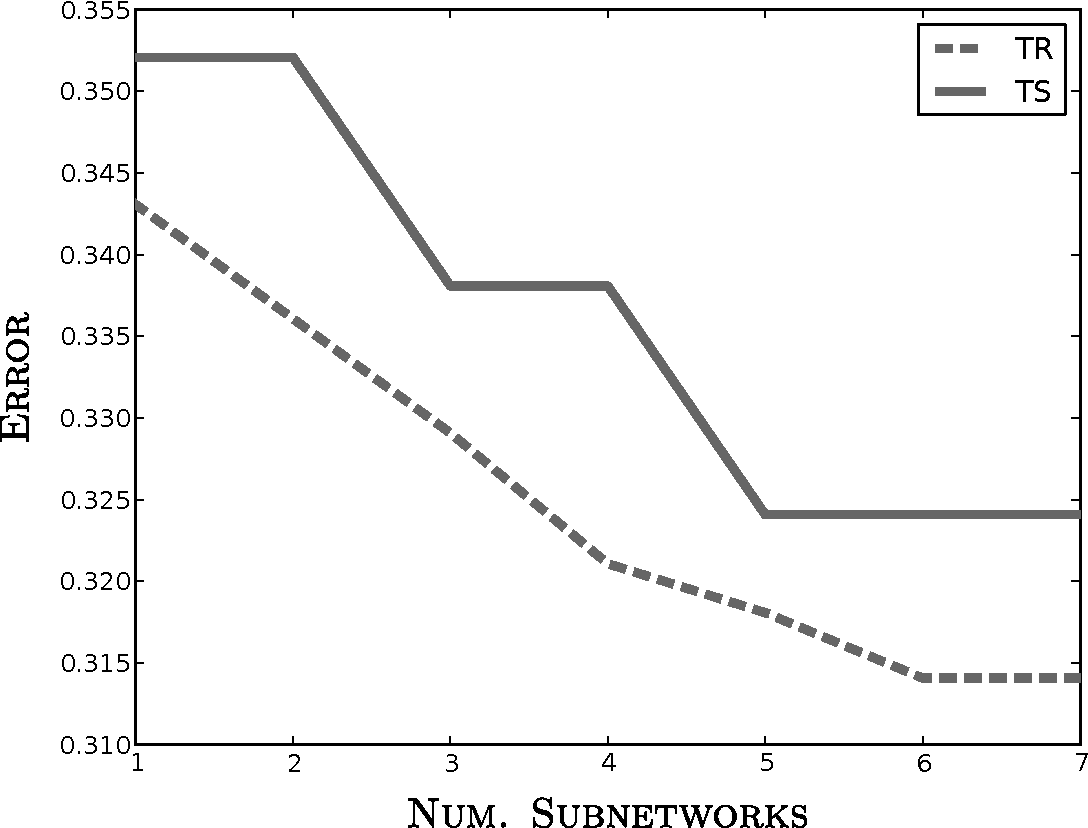
\includegraphics[width=0.5\columnwidth]{img/plot/ptc1}\\
\vspace*{0.8cm}
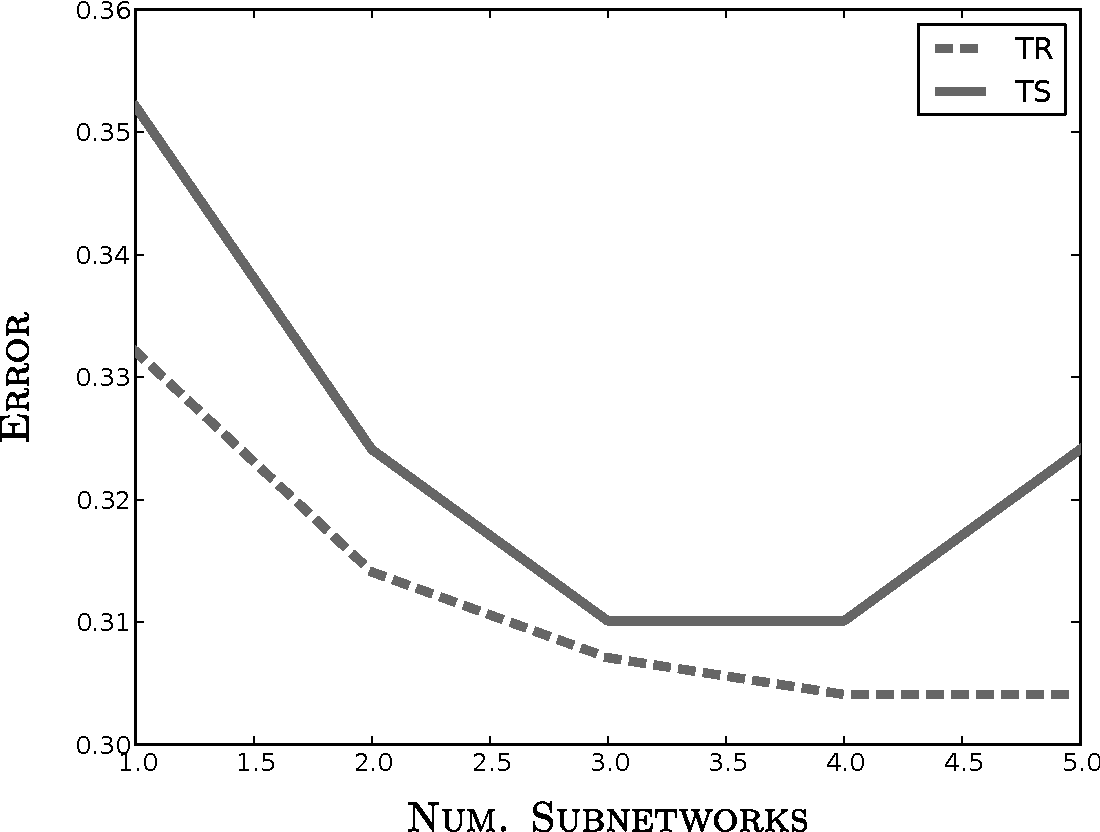
\includegraphics[width=0.5\columnwidth]{img/plot/ptc2}\\
\vspace*{0.8cm}
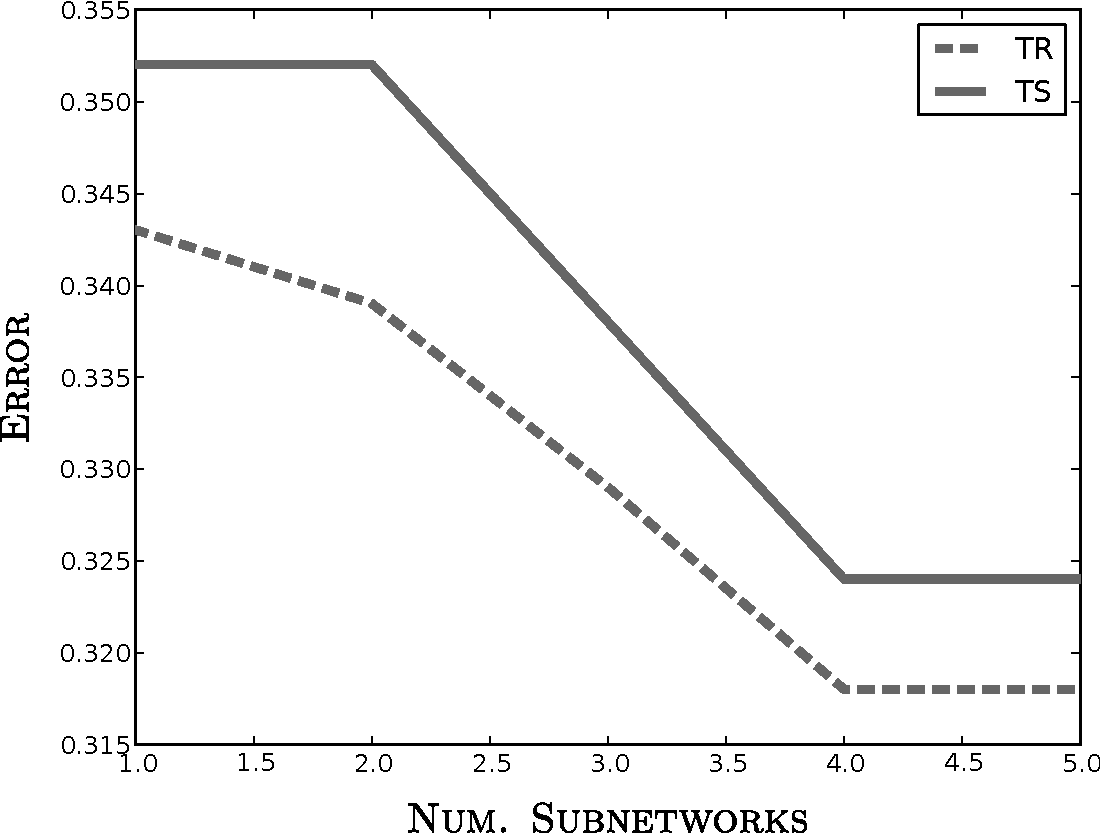
\includegraphics[width=0.5\columnwidth]{img/plot/ptc3}\\
\medskip
\caption[PTC: curve di apprendimento.]{GraphESN-FOF. Curve di apprendimento sul dataset PTC. Errore di misclassificazione commesso nel corso della costruzione della rete.\\
Linea tratteggiata: errore di training. Linea piena: errore di test.}
\label{fig:esperimenti:plot-ptc}
\end{figure}


L'accuratezza di predizione ottenuta tramite i modelli proposti risulta inoltre comparabile con quelle raggiunta applicando sugli stessi task dei modelli basati su kernel allo stato dell'arte nel trattamento dei domini strutturati \cite{Frohlich:OptimalAssignment}, riportati nella tabella~\ref{tab:esperimenti:kernelPTC}. Nel confronto è inoltre opportuno considerare che i modelli kernel-based prevedono, rispetto ai modelli proposti, l'impiego di maggiori risorse di calcolo ed operano attraverso l'impiego di metriche fissate a priori ed indipendenti dal task, in maniera simile a quanto avviene per i reservoir che non sfruttino output-feedback.
\begin{table}[tbp]
\small
\caption[Performance di metodi kernel-based su PTC]{Accuratezza media dei modelli e deviazione standard, in percentuale, di metodi basati su kernel applicati ai 4 task PTC.}
\label{tab:esperimenti:kernelPTC}
\centering
\begin{tabular}{l*{4}{c}}
\toprule
Method 	& FR	& FM	& MR	& MM	\\
\midrule
MG-Kernel & $70$ ($\pm 1$) & $65$ ($\pm 1$) & $63$ ($\pm 1$) & $69$ ($\pm 1$) \\
OA-Kernel & $70$ ($\pm 1$) & $65$ ($\pm 1$) & $63$ ($\pm 1$) & $68$ ($\pm 1$) \\
EM-Kernel & $69$ ($\pm 1$) & $65$ ($\pm 1$) & $61$ ($\pm 2$) & $67$ ($\pm 1$) \\
\bottomrule
\end{tabular}
\end{table}



%%%%%%%%%%%%%%%%%%%%%%%%%%%%%%%%%%%%%%
\subsection{Mutagenesis}
Le performance dei modelli sui tre task relativi al dataset Mutagenesis sono state calcolate ricorrendo ad una \emph{doppia k-fold cross-validation} (si veda il paragrafo~\ref{intro:validazione}) con un ciclo esterno di 10 fold ed un ciclo interno di 5 fold. La suddivisione del dataset è stata realizzata attraverso \emph{stratificazione} (si veda il paragrafo~\ref{intro:validazione}).
Per avere una stima più attendibile al variare dell'assegnazione iniziale dei pesi, 5 distinte ripetizioni sono state effettuate per ogni iperparametrizzazione testata.

Come nel caso di PTC, per ognuno dei modelli proposti sono state considerate due distinte configurazioni per la dimensione del reservoir delle sotto-reti: $N_R \in \lbrace 50, 30 \rbrace$. Il task structure-to-element di classificazione binaria, $N_Y = N_Z = 1$, prevede una dimensione delle etichette di input variabile, in base alla rappresentazione adottata: $N_U$ vale $11$, $13$, $15$ per AB, AB+C, AB+C+PS rispettivamente.

La soglia di convergenza del reservoir è stata fissata a $\epsilon = 10^{-5}$. Il coefficiente di contrazione $\sigma$ è stato in questo caso selezionato attraverso model selection.

Per interrompere la costruzione delle reti si è fissato $\delta_\textup{var} = 0.01$ e $\delta_\textup{tr} = 0.11$, riferito al miscalssification-rate. Come per PTC, il numero massimo di sotto-reti è stato fissato a $\delta_\textup{size} = 15$ nei casi in cui $N_R = 50$ e $\delta_\textup{size} = 20$ con $N_R = 30$.

Il learning-rate utilizzato per l'allenamento del readout globale tramite LMS è $\eta = 10^{-3}$.

La model selection è stata realizzata variando gli iperparametri $\lambda_\textup{in}$, $\lambda_\textup{fof}$, $\lambda_\textup{r}$,  $\lambda_\textup{wd}$ e $\sigma$, secondo i valori riportati nella tabella~\ref{tab:esperimenti:grigliaMutag}.
\begin{table}[tbp]
\small
\caption[Model selection: iperparametri per Mutagenesis]{Iperparametri usati per la model selection sui 3 task Mutagenesis.}
\label{tab:esperimenti:grigliaMutag}
\centering
\begin{tabular}{*{5}{c}}
\toprule
$\lambda_\textup{in}$ & $\lambda_\textup{fof}$ & $\lambda_\textup{r}$ & $\lambda_\textup{wd}$ & $\sigma$ \\
\midrule
$\lbrace 1.0, 0.1 \rbrace$ & $\lbrace 1.0, 2.0 \rbrace$ & $\lbrace 0.001, 0.01, 0.1 \rbrace$ & $\lbrace 0.0, 0.01 \rbrace$ &  $\lbrace 1.0, 2.0 \rbrace$\\
\bottomrule
\end{tabular}
\end{table}
Selezione e test del modello hanno dunque coinvolto, per i tre task e limitatamente ai casi costruttivi, l'allenamento di un totale di $72300$ diverse istanze di modello.

Sulle GraphESN la selezione degli iperparametri è stata eseguita facendo variare i valori di $N_R$, $\lambda_\textup{in}$, $\lambda_\textup{r}$ come indicato nella tabella~\ref{tab:esperimenti:grigliaMutagStandard}.
\begin{table}[tbp]
\small
\caption[Model selection: iperparametri per GraphESN su Mutag]{Iperparametri usati per la model selection di GraphESN sui 3 task Mutagenesis.}
\label{tab:esperimenti:grigliaMutagStandard}
\centering
\begin{tabular}{*{3}{c}}
\toprule
$N_R$ & $\lambda_\textup{in}$ & $\lambda_\textup{r}$ \\
\midrule
$\lbrace 500, 200, 100, 50 \rbrace$ & $\lbrace 1.0, 0.1 \rbrace$ & $\lbrace 0.01, 0.1, 0.2 \rbrace$ \\
\bottomrule
\end{tabular}
\end{table}

Nella tabella~\vref{tab:esperimenti:mutag} sono riportati i risultati sperimentali ottenuti sui tre task Mutagenesis.
I valori riportati rappresentano l'accuratezza percentuale di test (i.e.\ percentuale di grafi nel test-set classificata correttamente) mediata sulle $10$ fold e la deviazione standard media. Il dettaglio dei risultati sulle singole fold è riportato nelle tabelle~\ref{app:esp:Mutag-AB-CF}-\ref{app:esp:Mutag-ABCPC-FOF} (si veda l'appendice~\vref{app:esperimenti}).
\begin{table}[tbp]
\small
\caption[Accuratezza media su Mutagenesis]{Accuratezza media dei modelli e deviazione standard, in percentuale, sui 3 task Mutagenesis.}
\label{tab:esperimenti:mutag} 
\centering	
\begin{tabular}{l*{4}{c}}
\toprule
Model 		 & $N_R$& AB				  & AB+C			   & AB+C+PS	\\
\midrule
GraphESN 	 & 		& $75.2$ ($\pm 0.8$) & $76.5$ ($\pm 0.8$) & $80.3$ ($\pm 0.8$) \\
GraphESN-CF  & $50$ & $79.0$ ($\pm 2.3$) & $78.1$ ($\pm 1.8$) & $79.4$ ($\pm 0.5$) \\
GraphESN-CF  & $30$ & $79.6$ ($\pm 2.5$) & $76.0$ ($\pm 1.5$) & $79.7$ ($\pm 0.2$) \\
GraphESN-FW  & $50$ & $80.5$ ($\pm 2.8$) & $76.3$ ($\pm 2.0$) & $79.3$ ($\pm 1.8$) \\
GraphESN-FW  & $30$ & $79.7$ ($\pm 2.8$) & $76.7$ ($\pm 2.5$) & $80.6$ ($\pm 1.9$) \\
GraphESN-FOF & $50$ & $79.3$ ($\pm 3.6$) & $76.0$ ($\pm 2.8$) & $79.9$ ($\pm 1.9$) \\
GraphESN-FOF & $30$ & $76.8$ ($\pm 3.7$) & $77.0$ ($\pm 2.4$) & $80.0$ ($\pm 2.5$) \\
\bottomrule
\end{tabular}
\end{table}
Benché l'accuratezza nella predizione ottenuta dai modelli proposti risulti inferiore rispetto a quella raggiungibile con l'utilizzo di altri approcci (e.g.\ GNN \cite{Scarselli:GNN}), i risultati sperimentali evidenziano come i modelli costruttivi rappresentino una valida alternativa ed un miglioramento rispetto alle GraphESN.

Nella tabella~\ref{tab:dimensioni:mutag} sono riportati alcuni dati sulle dimensioni raggiunte delle reti nell'affrontare i tre task del dataset.
\begin{table}
\small
\caption[Dimensioni delle reti su Mutagenesis]{Numero di sotto-reti dei modelli sui tre task Mutagenesis. Numero massimo, numero minimo, media e moda.}
\label{tab:dimensioni:mutag} 
\centering	
\begin{tabular}{l*{4}{c}}
\toprule
Model 		 & Max & Min & Avg & Mode \\
\midrule
GraphESN-CF  & $17$ & $2$ & $3.9$ & $2$ \\
GraphESN-FW  & $15$ & $2$ & $4.6$ & $2$ \\
GraphESN-FOF & $18$ & $2$ & $5.5$ & $4$ \\
\bottomrule
\end{tabular}
\end{table}
In questo caso la tabella evidenzia la presenza di molte reti di dimensioni minime, suggerendo l'adozione di un criterio di stop più sofisticato per interrompere la costruzione della rete. La condizione di arresto utilizzata guarda infatti al solo errore di training commesso al passo precedente e, nel caso di task complessi, è ipotizzabile che questo possa non essere sufficiente a determinare l'effettivo andamento del processo di learning. Criteri di stop più sofisticati potrebbero, ad esempio, usare un validation-set per determinare la dimensione ottimale della rete.

La figura~\vref{fig:esperimenti:plot-mutag} mostra un esempio di alcune curve di apprendimento che caratterizzano l'applicazione dei modelli sul dataset. Il valore di errore indicato è il misclassification-rate. La figura evidenzia come l'errore di test diminuisca al decrescere dell'errore di training, e dunque come il processo di apprendimento costruttivo abbia effettivamente la capacità di migliorare la capacità predittiva del modello. Si riscontra tuttavia uno scostamento piuttosto ampio fra l'errore commesso sui dati training e quello commesso sui dati di test, che suggerisce l'opportunità di perfezionare i risultati ottenuti adottando ulteriori criteri di regolarizzazione, che riducano la complessità della rete.
\begin{figure}[p]
\centering
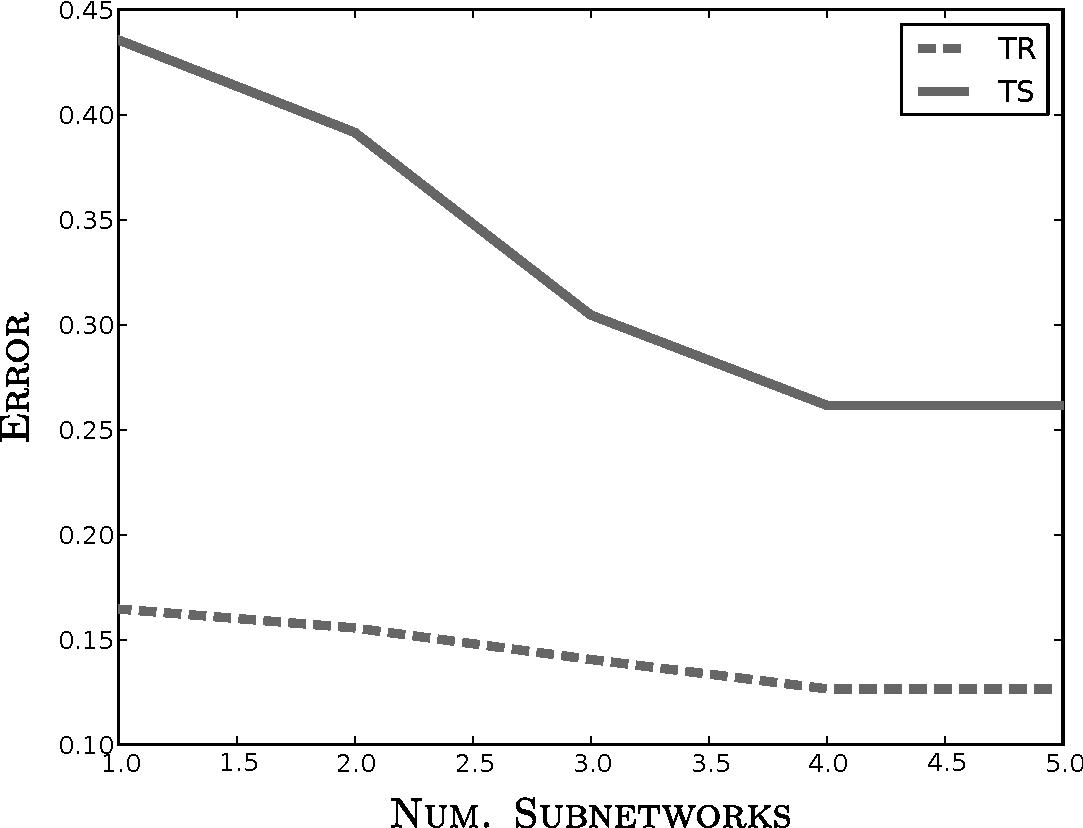
\includegraphics[width=0.5\columnwidth]{img/plot/mutag1}\\
\vspace*{0.8cm}
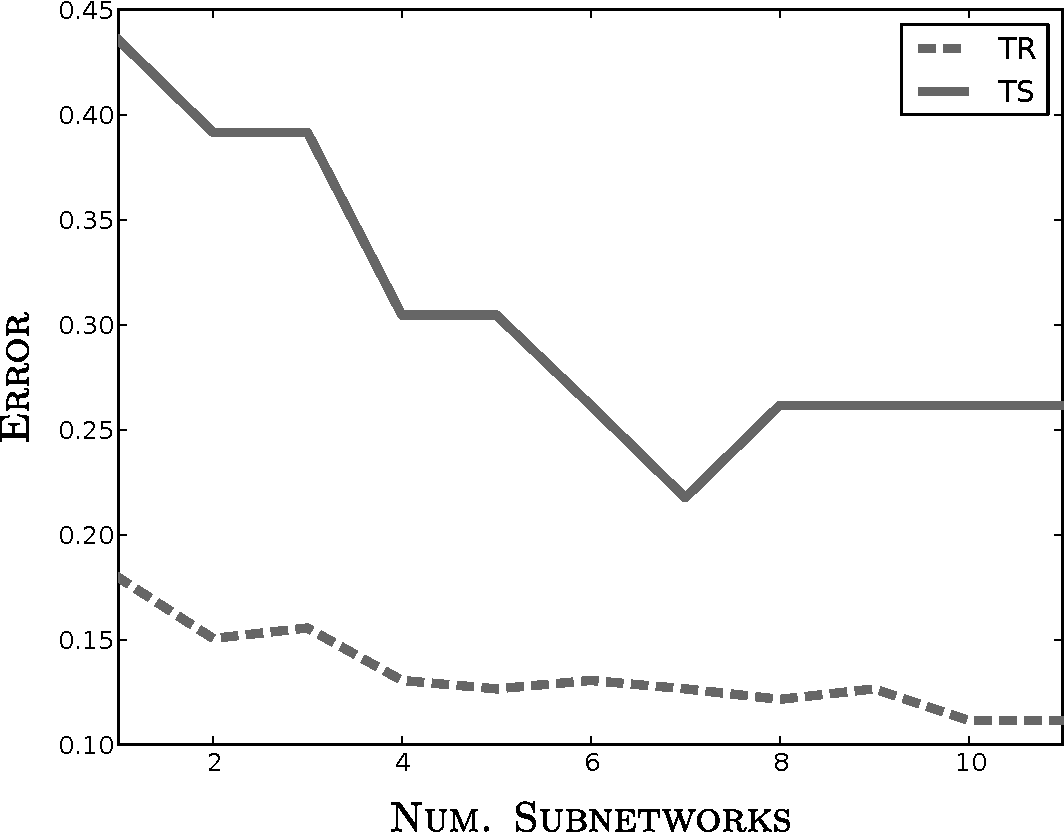
\includegraphics[width=0.5\columnwidth]{img/plot/mutag2}\\
\vspace*{0.8cm}
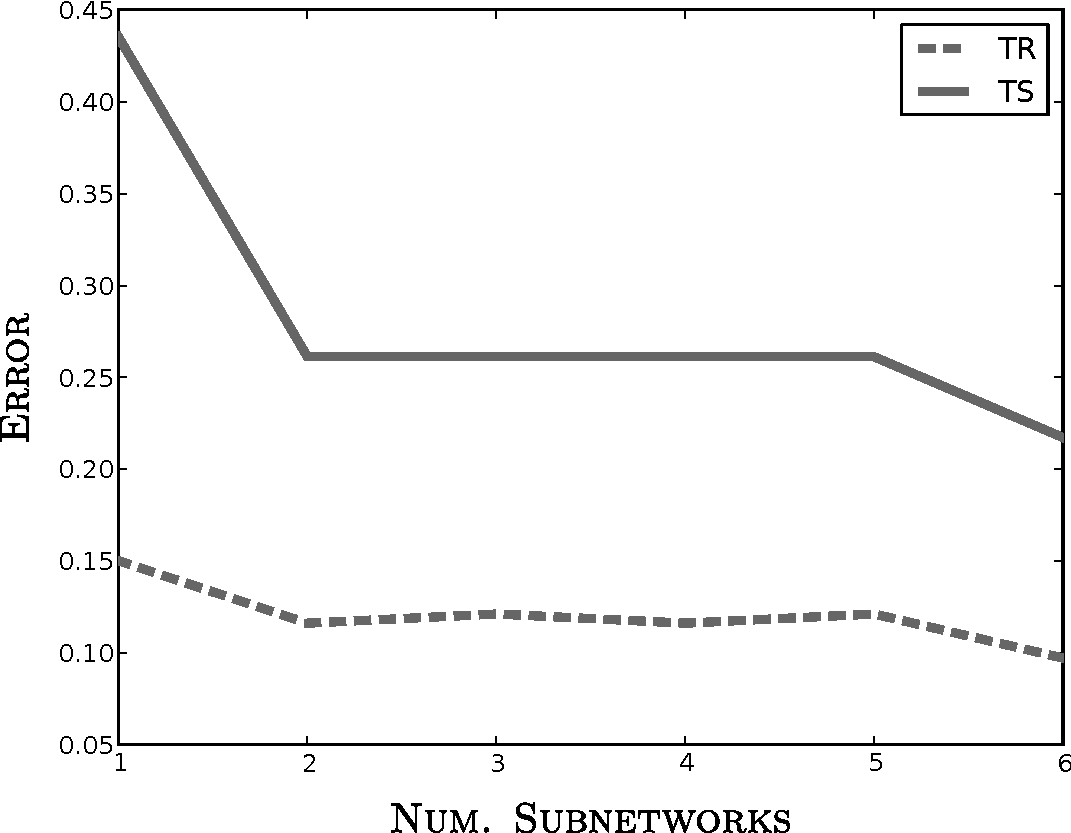
\includegraphics[width=0.5\columnwidth]{img/plot/mutag3}\\
\medskip
\caption[Mutag: curve di apprendimento.]{GraphESN-FOF. Curve di apprendimento sul dataset Mutagenesis. Errore di misclassificazione commesso nel corso della costruzione della rete.\\
Linea tratteggiata: errore di training. Linea piena: errore di test.}
\label{fig:esperimenti:plot-mutag}
\end{figure}

 

%%%%%%%%%%%%%%%%%%%%%%%%%%%%%%%%%%%%%%
\subsection{Bursi}
Sul dataset Bursi è stato possibile sfruttare una suddivisione preesistente del dataset in dati di training e dati di test. La selezione del modello è stata dunque realizzata suddividendo il training-set in $5$ fold tramite stratificazione e realizzando una \emph{k-fold cross-validation} con dei validation-set per selezionare gli iperparametri (si veda il paragrafo~\ref{intro:validazione}). Successivamente si è usato il partizionamento originale del dataset, in trainig-set e test-set, per testare le capacità predittive dei modelli. La suddivisione in fold è avvenuta ricorrendo a \emph{stratificazione} (si veda il paragrafo~\ref{intro:validazione}). Per ogni iperparametrizzazione testata sono state effettuate 5 ripetizioni distinte, in modo da variare l'assegnazione iniziale dei pesi.

Sul dataset sono stati testati modelli costruttivi con sotto-reservoir di dimensione $N_R = 100$. Il task structure-to-element di classificazione binaria $N_Y = N_Z = 1$ prevede una dimensione delle etichette di input $N_U = 14$.

La soglia di convergenza del reservoir utilizzata è $\epsilon = 10^{-5}$, mentre il coefficiente di contrazione è stato fissato a $\sigma = 1.0$.

Per interrompere la costruzione delle reti si è fissato $\delta_\textup{var} = 0.01$ e $\delta_\textup{tr} = 0.15$, riferito al miscalssification-rate, con un numero massimo di sotto-reti consentito $\delta_\textup{size} = 10$.

Il learning-rate $\eta = 10^{-3}$ è stato utilizzato per l'allenamento del readout globale tramite LMS.

Data la dimensione del dataset, ed il relativo onere computazionale, la model selection su Bursi ha interessato i soli iperparametri $\lambda_\textup{fof}$ e $\lambda_\textup{r}$, mantenendo fissi i parametri $\lambda_\textup{wd} = 0$ per l'apprendimento nel readout globale e $\lambda_\textup{in} = 1.0$ per lo scaling dei pesi dall'input.
I valori degli iperparametri coinvolti nella model selection sono riportati nella tabella~\ref{tab:esperimenti:grigliaBursi}.
\begin{table}[tbp]
\small
\caption[Model selection: iperparametri per Bursi]{Iperparametri usati per la model selection su Bursi.}
\label{tab:esperimenti:grigliaBursi}
\centering
\begin{tabular}{*{2}{c}}
\toprule
$\lambda_\textup{fof}$ & $\lambda_\textup{r}$ \\
\midrule
$\lbrace 1.0, 2.0 \rbrace$ & $\lbrace 0.0, 0.001, 0.01, 0.1 \rbrace$ \\
\bottomrule
\end{tabular}
\end{table}
%
Le performance su GraphESN sono invece state calcolate facendo variare i parametri $N_R$ e $\lambda_\textup{r}$ in accordo ai valori riportati nella tabella~\ref{tab:esperimenti:grigliaBursiStandard}.
\begin{table}[tbp]
\small
\caption[Model selection: iperparametri per GraphESN su Bursi]{Iperparametri usati per la model selection di GraphESN su Bursi.}
\label{tab:esperimenti:grigliaBursiStandard}
\centering
\begin{tabular}{*{2}{c}}
\toprule
$N_R$ & $\lambda_\textup{r}$ \\
\midrule
$\lbrace 500, 200, 100 \rbrace$ & $\lbrace 0.0, 0.001, 0.01, 0.1 \rbrace$ \\
\bottomrule
\end{tabular}
\end{table}
%
Gli esperimenti sul dataset hanno dunque richiesto l'allenamento complessivo di $680$ diverse reti.

I risultati sperimentali ottenuti sono riportati nella tabella~\ref{tab:esperimenti:bursi}, con i valori ad indicare l'accuratezza percentuale e la deviazione standard riscontrate nel classificare i dati sia di training che di test.
\begin{table}[tbp]
\small
\caption[Accuratezza media su Bursi]{Accuratezza media in training e test dei modelli e deviazione standard, in percentuale, sul dataset Bursi.}
\label{tab:esperimenti:bursi} 
\centering	
\begin{tabular}{l*{3}{c}}
\toprule
Model           & $N_R$     & TR                    & TS        \\
\midrule
GraphESN        &           & $77.9$ ($\pm 0.2$)    & $76.2$ ($\pm 0.2$) \\
GraphESN-CF     & $100$     & $78.3$ ($\pm 0.4$)    & $76.7$ ($\pm 0.7$) \\
GraphESN-FW     & $100$     & $78.4$ ($\pm 0.8$)    & $77.1$ ($\pm 0.7$) \\
GraphESN-FOF    & $100$     & $79.8$ ($\pm 0.5$)    & $78.0$ ($\pm 0.9$) \\
\bottomrule
\end{tabular}
\end{table}
Dai dati emerge come in questo caso l'approccio costruttivo permetta di superare sistematicamente le performance predittive ottenute tramite GraphESN. Risulta inoltre come il miglioramento delle performance segua l'arricchimento della connettività progressivo realizzato dai tre modelli costruttivi.

La tabella~\ref{tab:dimensioni:mutag} riporta i dati sulle dimensioni raggiunte delle reti nell'affrontare il task.
\begin{table}
\small
\caption[Dimensioni delle reti su Bursi]{Numero di sotto-reti dei modelli su Bursi. Numero massimo, numero minimo, media e moda.}
\label{tab:dimensioni:bursi} 
\centering	
\begin{tabular}{l*{4}{c}}
\toprule
Model 		 & Max & Min & Avg & Mode \\
\midrule
GraphESN-CF  & $5$ & $2$ & $3.2$ & $2$ \\
GraphESN-FW  & $8$ & $2$ & $4.2$ & $4$ \\
GraphESN-FOF & $10$ & $4$ & $6.8$ & $7$ \\
\bottomrule
\end{tabular}
\end{table}
Si nota come il modello GraphESN-FOF riesca a procedere più a lungo nella costruzione della rete, probabilmente grazie ad una maggiore capacità di fitting che permette all'errore sul trainig-set di variare maggiormente, senza determinare l'interruzione del processo di costruzione della rete.

La figura~\vref{fig:esperimenti:plot-bursi} mostra un esempio dell'andamento del training di una rete di tipo GraphESN-FOF applicata al dataset, evidenziando il progresso della capacità predittiva della rete nel corso del procedimento di costruzione della rete.
\begin{figure}[p]
\centering
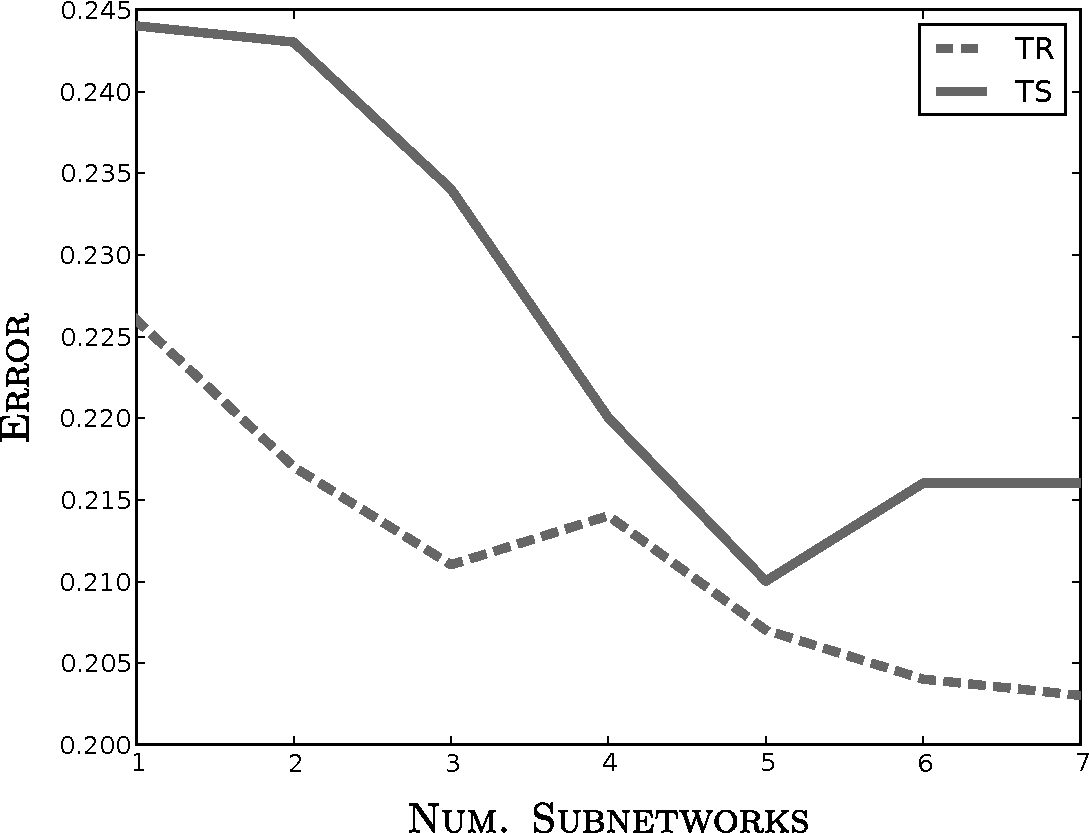
\includegraphics[width=0.7\columnwidth]{img/plot/bursi}
\medskip
\caption[Bursi: curve di apprendimento.]{GraphESN-FOF. Curve di apprendimento sul dataset Bursi. Errore di misclassificazione commesso nel corso della costruzione della rete.\\
Linea tratteggiata: errore di training. Linea piena: errore di test.}
\label{fig:esperimenti:plot-bursi}
\end{figure}


%%%%%%%%%%%%%%%%%%%%%%%%%%%%%%%%%%%%%%
\subsection{Angiotensin Converting Enzyme}
Sul dataset ACE non è stato svolto un processo di selezione degli iperparametri ottimali dei modelli, limitando l'analisi sperimentale ad una singola iperparametrizzazione, scelta sulla base di valutazioni empiriche. La valutazione della performance del modello è stata svolta attraverso \emph{k-fold cross-validation} su $10$ fold (si veda il paragrafo~\ref{intro:validazione}), ripetendo il test $5$ volte in modo da variare l'inizializzazione dei pesi di reservoir.

Il dataset ACE ha permesso di applicare i modelli ad un task structure-to-element di regressione, con $N_Y = N_Z = 1$. Le etichette associate ai vertici dell'input risultano avere dimensione $N_U = 8$.

Per interrompere il processo di encoding è stata usata la soglia $\epsilon = 10^{-5}$, fissando un coefficiente di contrazione per ogni reservoir $\sigma = 1.0$.

Il processo di costruzione della rete è stato interrotto fissando $\delta_\textup{var} = 0.01$ e senza tenere conto di alcun errore minimo sul training-set, $\delta_\textup{tr} = -1.0$, con un numero massimo di sotto-reti consentito pari a $\delta_\textup{size} = 30$.

L'allenamento del readout globale è stato svolto attraverso LMS con learning-rate $\eta = 10^{-3}$ e senza applicare alcun fattore di weight-decay, $\lambda_\textup{wd} = 0$.
L'apprendimento nelle sotto-reti è stato realizzato attraverso una Ridge Regression con fattore di regolarizzazione $\lambda_\textup{r} = 0.1$.

Per l'inizializzazione dei pesi sono stati fissati i parametri $\lambda_\textup{in} = 1.0$ e $\lambda_\textup{fof} = 2.0$. 
Il test è stato svolto utilizzando sotto-reti di dimensione $N_R = 30$.

Per poter effettuare un confronto, l'allenamento su GraphESN è stato eseguito mantenendo, laddove abbia un senso, la stessa iperparametrizzazione usata per i modelli costruttivi. La dimensione del reservoir in questo caso è però stata fatta variare $N_R \in \lbrace 90, 150, 300, 450 \rbrace$. Nel seguito viene riportato solo il risultato migliore ottenuto (i.e.\ $N_R = 300$), in termini di performance predittiva.

La tabella~\ref{tab:esperimenti:ACE} mostra i risultati sperimentali ottenuti, indicando l'errore quadratico medio e la deviazione standard mediati sulle $10$ fold.
\begin{table}[tb]
\small
\caption[Accuratezza media su ACE]{Errore quadratico medio in training e test dei modelli e deviazione standard sul dataset ACE.}
\label{tab:esperimenti:ACE}
\centering
\begin{tabular}{l*{2}{c}}
\toprule
Model & MSE (TR) & MSE (TS) \\
\midrule
GraphESN    & $1.83$ ($\pm 0.01$) &	$2.13$ ($\pm 0.03$) \\ 
GraphESN-CF & $2.03$ ($\pm 0.07$) & $2.37$ ($\pm 0.15$) \\
GraphESN-FW & $1.71$ ($\pm 0.02$) & $2.02$ ($\pm 0.06$) \\
GraphESN-FOF & $1.60$ ($\pm 0.07$) & $2.03$ ($\pm 0.06$) \\
\bottomrule
\end{tabular}
\end{table}
%
Benché non sia stata effettuata una selezione rigorosa degli iperparametri ottimali per il task, è importante sottolineare come i risultati ottenuti siano comparabili con quelli riportati in letteratura relativamente all'applicazione di altri modelli per l'apprendimento di trasduzioni strutturali.
La tabella~\ref{tab:esperimenti:kernelACE} indica le performance su ACE ottenute attraverso modelli basati su kernel allo stato dell'arte nel trattamento di domini strutturati \cite{Hinselmann:GraphKernels}.
\begin{table}[tbp]
\small
\caption[Performance di metodi kernel-based su ACE]{Errore quadratico medio dei modelli e deviazione standard di metodi basati su kernel sul dataset ACE.}
\label{tab:esperimenti:kernelACE}
\centering
\begin{tabular}{lc}
\toprule
Kernel 	& MSE \\
\midrule
DotProduct & $1.60$ ($\pm 0.59$) \\
2D-LAP(CK) & $1.67$ ($\pm 0.63$) \\
2D-LAP(OA) & $1.81$ ($\pm 0.65$) \\
3D-LAP(CK) & $2.04$ ($\pm 0.78$) \\
3D-LAP(OA) & $1.91$ ($\pm 0.71$) \\
XD-LAP(CK) & $1.90$ ($\pm 0.71$) \\
XD-LAP(OA) & $1.99$ ($\pm 0.71$) \\
MACCS keys & $2.02$ ($\pm 0.69$) \\
Marginalized GK & $1.74$ ($\pm 0.72$) \\
Pharmacophore & $2.24$ ($\pm 0.82$) \\
OAK & $1.49$ ($\pm 0.68$) \\
Tanimoto DFS & $1.85$ ($\pm 0.64$) \\
\bottomrule
\end{tabular}
\end{table}

La figura~\vref{fig:esperimenti:plot-ace} riporta una campione delle curve di apprendimento ottenute utilizzando una rete di tipo GraphESN-FOF sul dataset. I grafici dimostrano l'efficacia del processo di apprendimento, mostrando tuttavia come la mancanza della scelta di un setting specifico su ogni fold risulti in un comportamento non uniforme dei modelli sulle varie fold.
\begin{figure}[p]
\centering
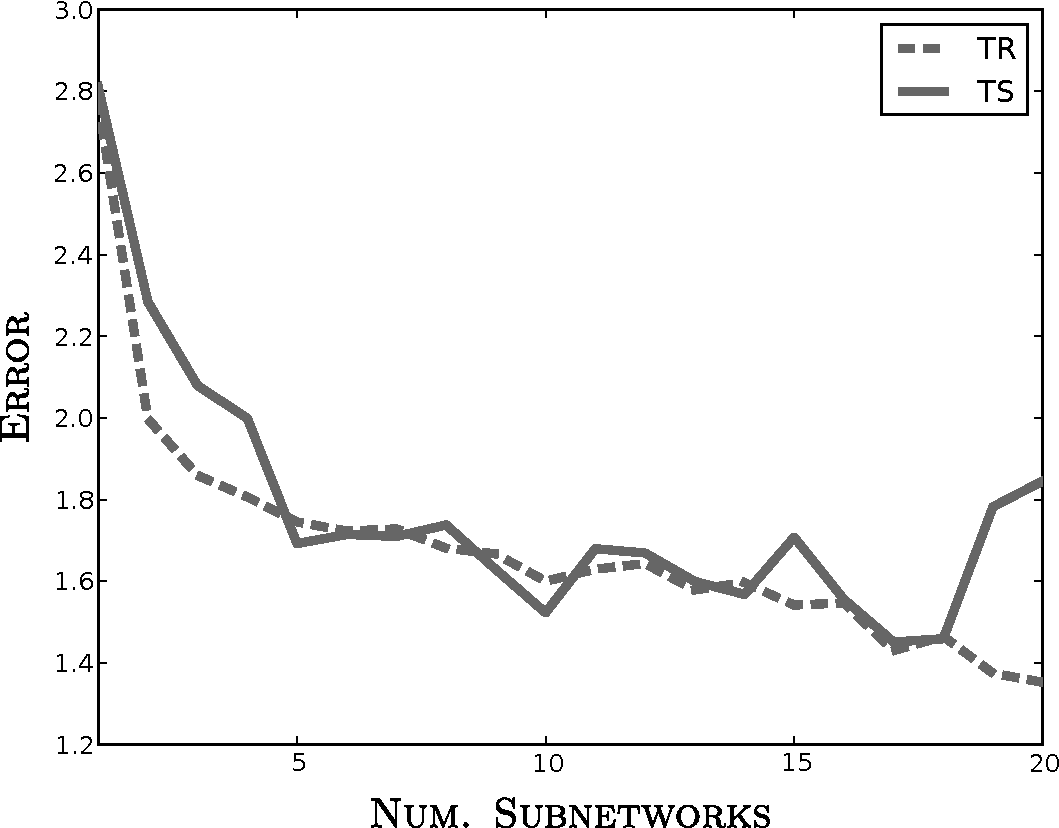
\includegraphics[width=0.5\columnwidth]{img/plot/ace1}\\
\vspace*{0.8cm}
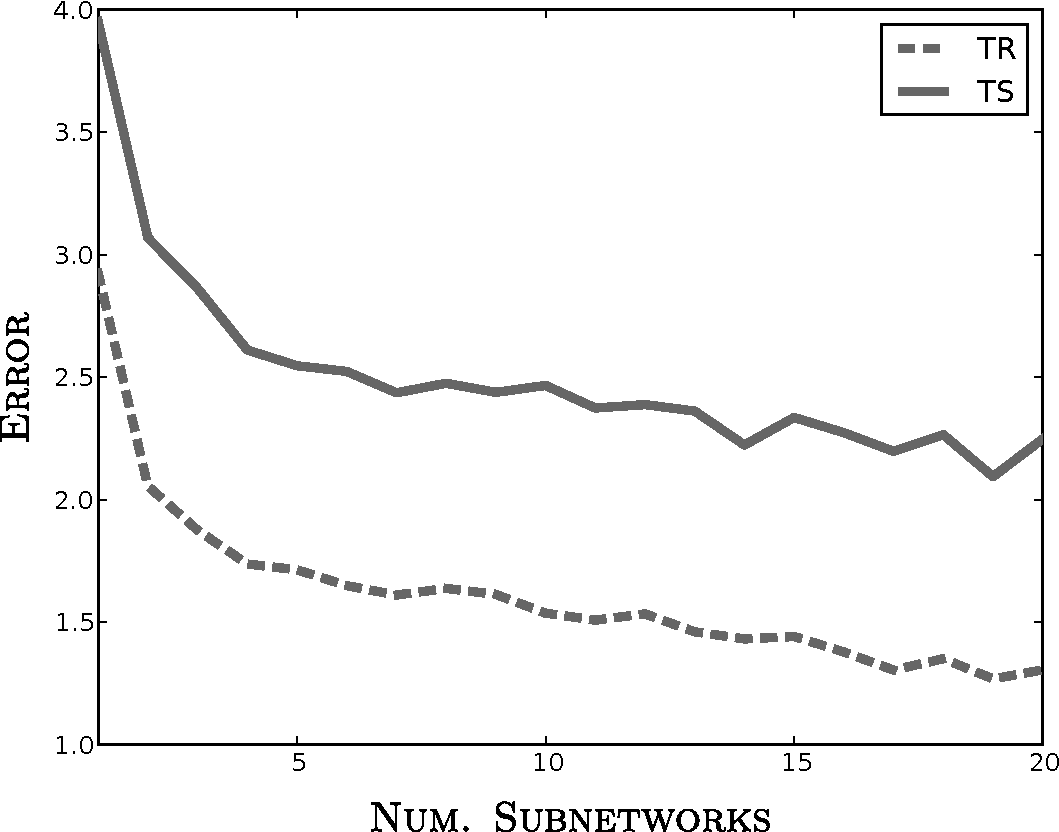
\includegraphics[width=0.5\columnwidth]{img/plot/ace2}\\
\vspace*{0.8cm}
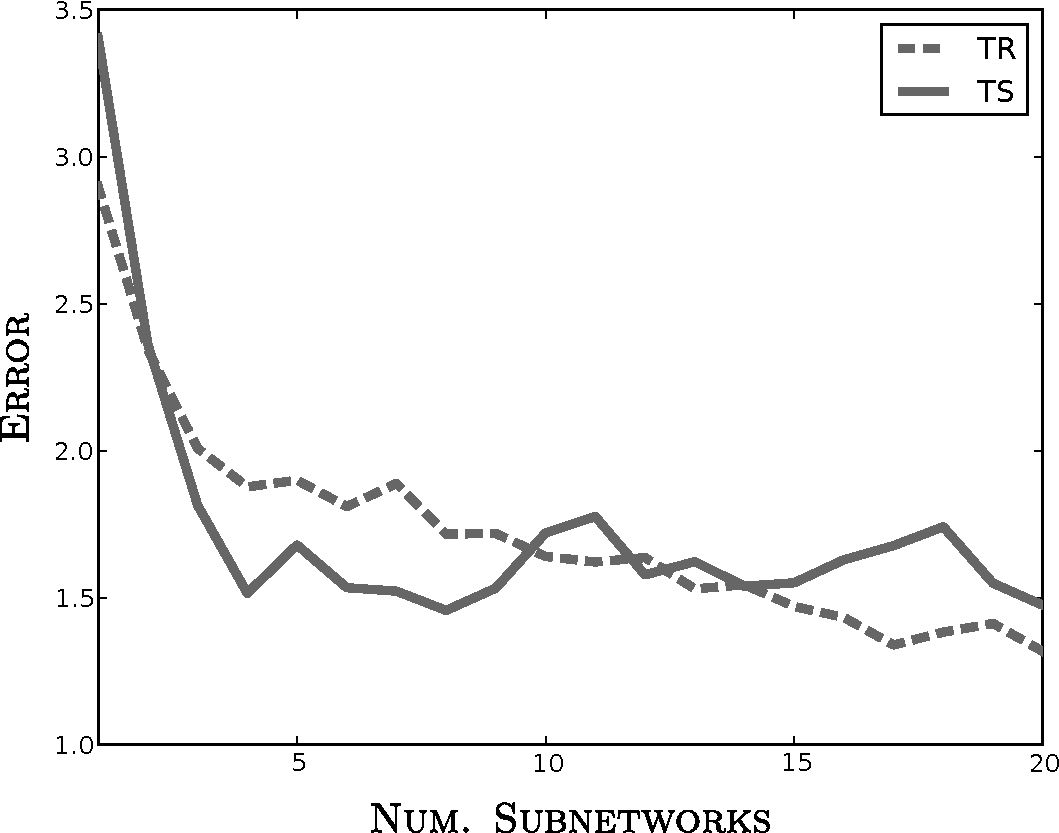
\includegraphics[width=0.5\columnwidth]{img/plot/ace3}\\
\medskip
\caption[ACE: curve di apprendimento.]{GraphESN-FOF. Curve di apprendimento sul dataset ACE. Errore quadratico medio (MSE) commesso nel corso della costruzione della rete.\\
Linea tratteggiata: errore di training. Linea piena: errore di test.}
\label{fig:esperimenti:plot-ace}
\end{figure}


%%%%%%%%%%%%%%%%%%%%%%%%%%%%%%%%%%%%%%
\section{Considerazioni}\label{sec:esperiment:considerazioni}
Guardando ai risultati emerge piuttosto chiaramente come la strategia costruttiva, seppur meno onerosa dal punto di vista computazionale, possa rappresentare un potenziamento delle GraphESN. Sia la fase di training che la selezione del modello si avvalgono infatti dell'approccio costruttivo per ridurre il costo computazionale senza che questo determini una perdita nella capacità predittiva della rete: i risultati ottenuti mostrano infatti come i modelli proposti siano in grado di superare nella maggior parte dei casi le performance raggiunte da GraphESN, raggiungendo risultati comparabili negli altri casi. In quest'ottica i modelli introdotti si configurano come uno strumento utile nel trattamento dei domini strutturati, in grado di soddisfare efficacemente i vincoli imposti dalla presenza di risorse di calcolo o di tempo limitate.

Guardando alla sola analisi delle performance, tuttavia, alcune caratteristiche dei modelli proposti rimangono poco chiare. Si nota ad esempio come l'introduzione e lo sfruttamento di un meccanismo stabile di output-feedback, nel modello GraphESN-FOF, non corrisponda ad un miglioramento sistematico dell'accuratezza predittiva della rete. Ulteriori analisi sperimentali hanno tuttavia permesso di verificare l'effetto dei segnali di output-feedback sui reservoir delle sotto-reti.
L'organizzazione dello spazio degli stati dei reservoir è stata investigata attraverso la Principal Component Analysis (PCA) \cite{Jolliffe:PCA}. La figura~\vref{fig:esperimenti:pca-ptc-fof} mostra le prime due componenti principali dello spazio degli stati dei reservoir di sotto-reti appartenenti ad una GraphESN-FOF. I punti dei plot corrispondono ai grafi in input, colorati in base al target loro assegnato e disposti nello spazio delle features secondo l'encoding corrispondente. Lo stesso procedimento e lo stesso setting sperimentale sono stati utilizzati per realizzare la figura~\vref{fig:esperimenti:pca-ptc-nofof}, che mostra lo spazio degli stati dei reservoir di una rete di tipo GraphESN-CF, in cui non sono presenti connessioni di output-feedback. Dal confronto delle due figure emerge chiaramente come il meccanismo di output-feedback abbia l'effetto di modificare le dinamiche del processo di encoding, organizzando gli input nello spazio degli stati in maniera coerente con il task affrontato ed aumentando progressivamente la distanza fra input appartenenti a classi distinte. 
%
\begin{figure}[p]
\centering
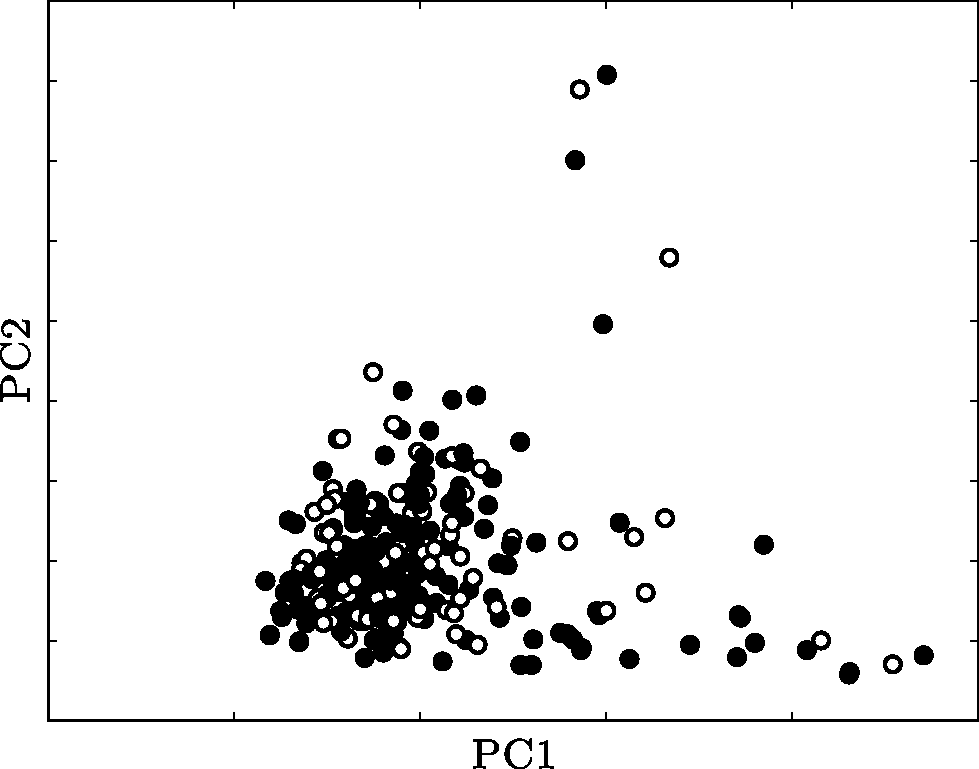
\includegraphics[width=0.5\columnwidth]{img/pca/pca-ptc-fof1}\\
\vspace*{0.8cm}
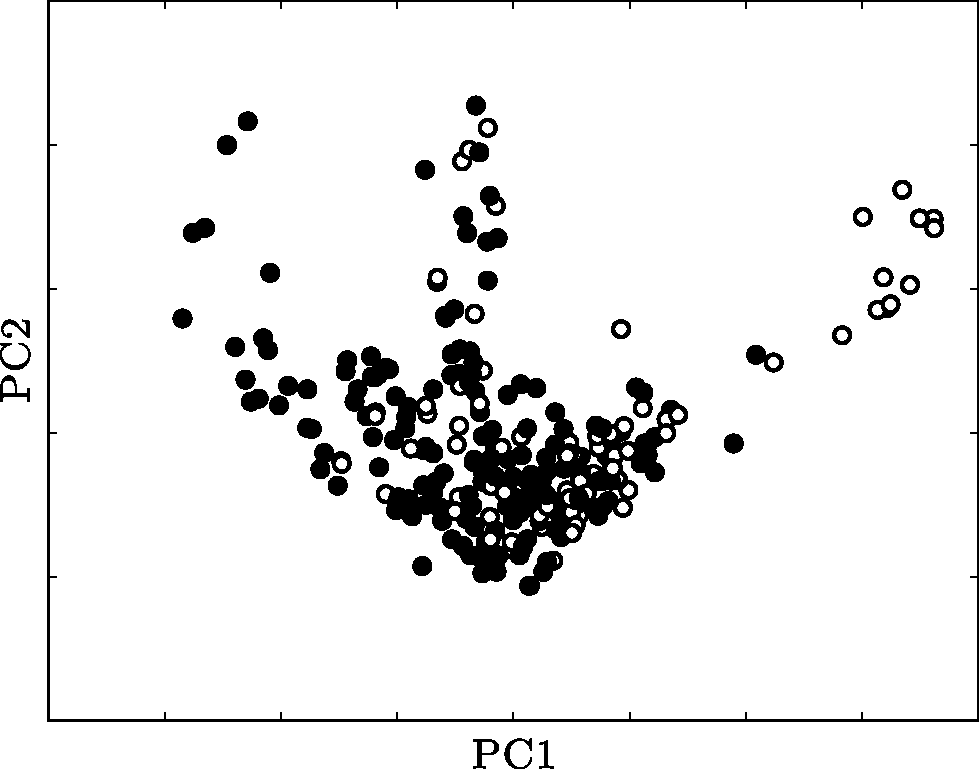
\includegraphics[width=0.5\columnwidth]{img/pca/pca-ptc-fof2}\\
\vspace*{0.8cm}
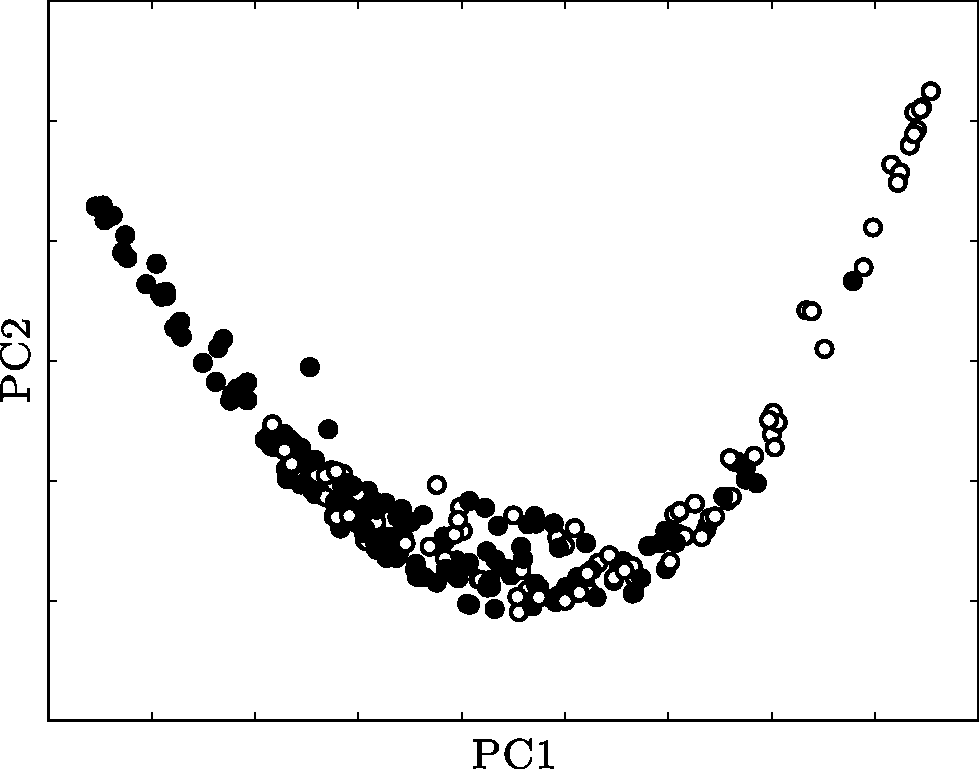
\includegraphics[width=0.5\columnwidth]{img/pca/pca-ptc-fof3}\\
\medskip
\caption[PCA dei reservoir. GraphESN-FOF su PTC-FR.]{Plot delle prime due componenti principali dello spazio degli stati dei reservoir nelle sotto-reti. Modello GraphESN-FOF applicato al task PTC-FR.\\ 
In nero: gli input con target $-1$. In bianco: gli input con target $+1$.\\
Reservoir riportati: (\emph{alto}) sotto-rete 1; (\emph{centro}) sotto-rete 5; (\emph{basso}) sotto-rete 9.}
\label{fig:esperimenti:pca-ptc-fof}
\end{figure}
%
\begin{figure}[p]
\centering
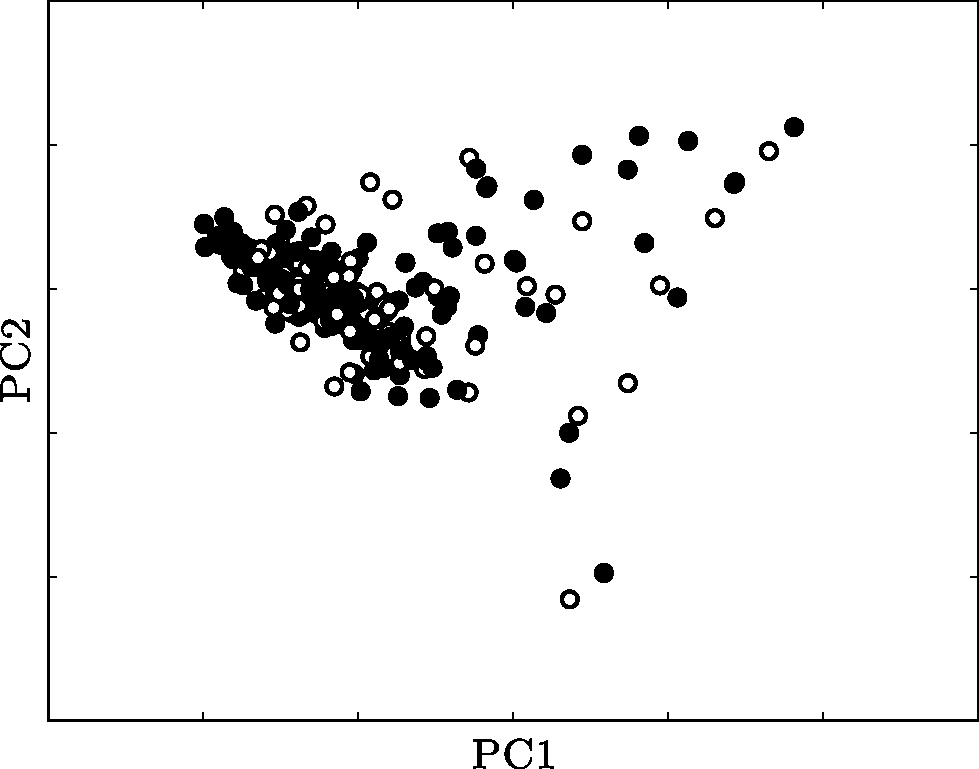
\includegraphics[width=0.5\columnwidth]{img/pca/pca-ptc-nofof1}\\
\vspace*{0.8cm}
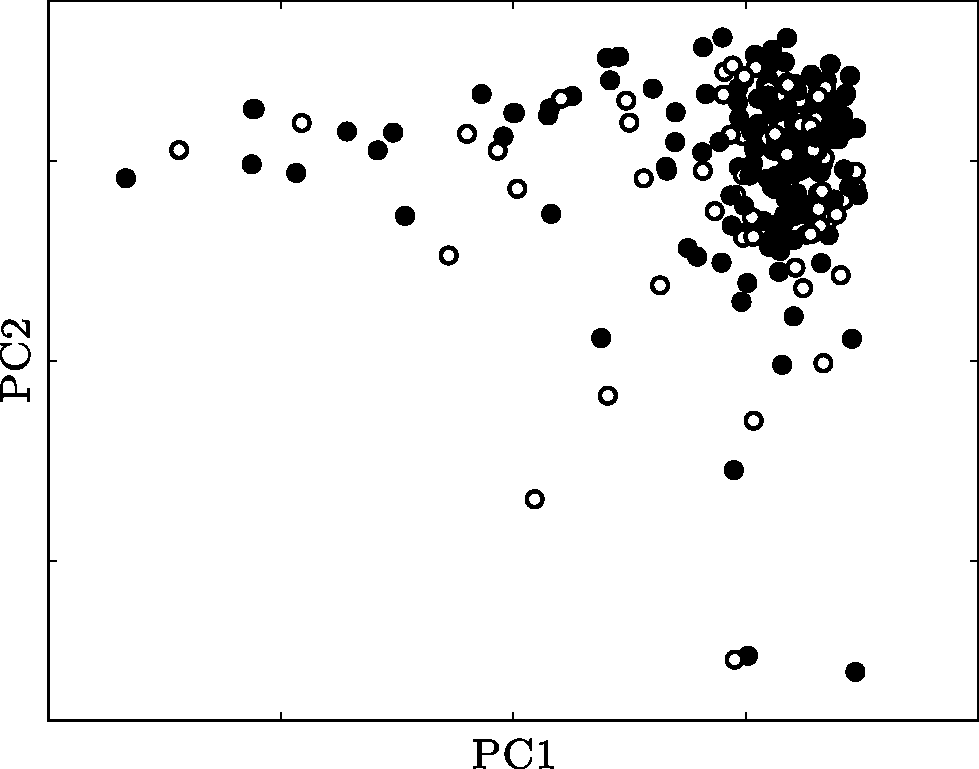
\includegraphics[width=0.5\columnwidth]{img/pca/pca-ptc-nofof2}\\
\vspace*{0.8cm}
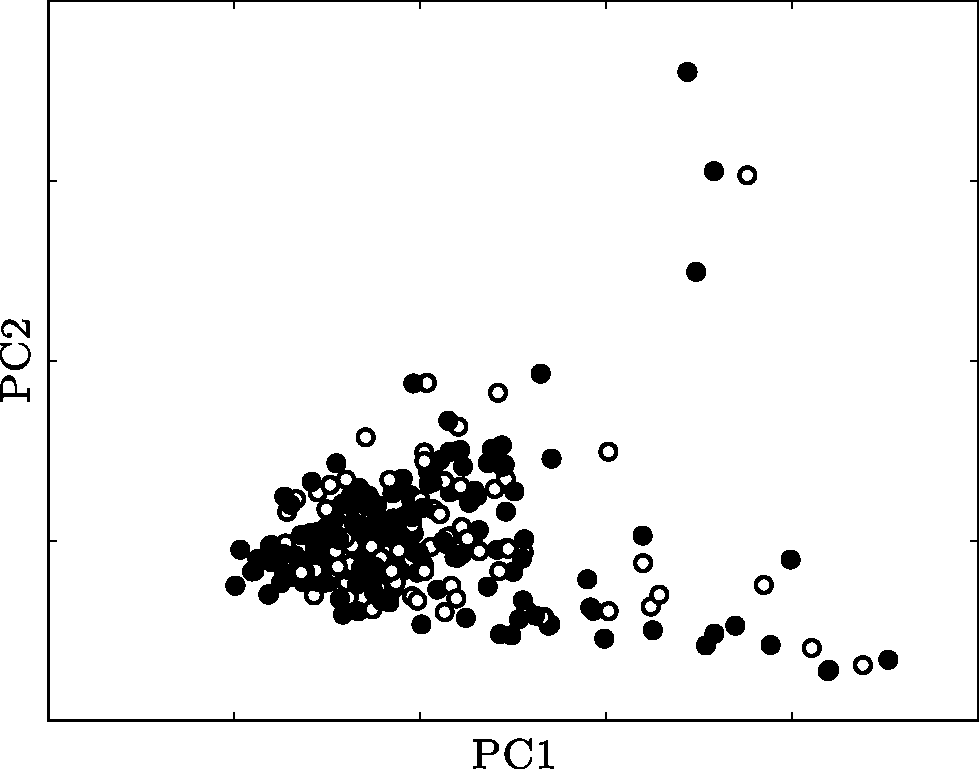
\includegraphics[width=0.5\columnwidth]{img/pca/pca-ptc-nofof3}\\
\medskip
\caption[PCA dei reservoir. GraphESN-CF su PTC-FR.]{Plot delle prime due componenti principali dello spazio degli stati dei reservoir nelle sotto-reti. Modello GraphESN-CF applicato al task PTC-FR.\\ 
In nero: gli input con target $-1$. In bianco: gli input con target $+1$.\\
Reservoir riportati: (\emph{alto}) sotto-rete 1; (\emph{centro}) sotto-rete 4; (\emph{basso}) sotto-rete 8.}
\label{fig:esperimenti:pca-ptc-nofof}
\end{figure}
%
\\
L'analisi della PCA è stata ripetuta sul dataset ACE, corrispondente ad un task di regressione. La figura~\vref{fig:esperimenti:pca-ace-fof} mostra lo spazio degli stati di una rete GraphESN-FOF, mentre la figura~\ref{fig:esperimenti:pca-ace-nofof} si riferisce ad una rete GraphESN-CF con lo stesso setting. Gli input sono in questo caso colorati in scale di grigio in accordo al valore target corrispondente, che varia in un intervallo continuo.
Anche in questo caso le figure evidenziano come la presenza di output-feedback abbia l'effetto di organizzare la rappresentazione dell'input all'interno dello spazio degli stati in maniera consistente con il task. Al contrario, nei due casi visti, l'assenza di output-feedback fa sì che i reservoir delle varie sotto-reti si comportino in maniera sostanzialmente simile l'uno all'altro, con variazioni dell'encoding che dipendono unicamente dalla diversa inizializzazione random dei pesi sulle connessioni ricorrenti.\\
Dall'analisi della PCA sugli stati dei reservoir risulta quindi ben evidente come la presenza degli output-feedback introduca effettivamente dell'informazione supervisionata all'interno di reservoir non adattivi.
%
\begin{figure}[p]
\centering
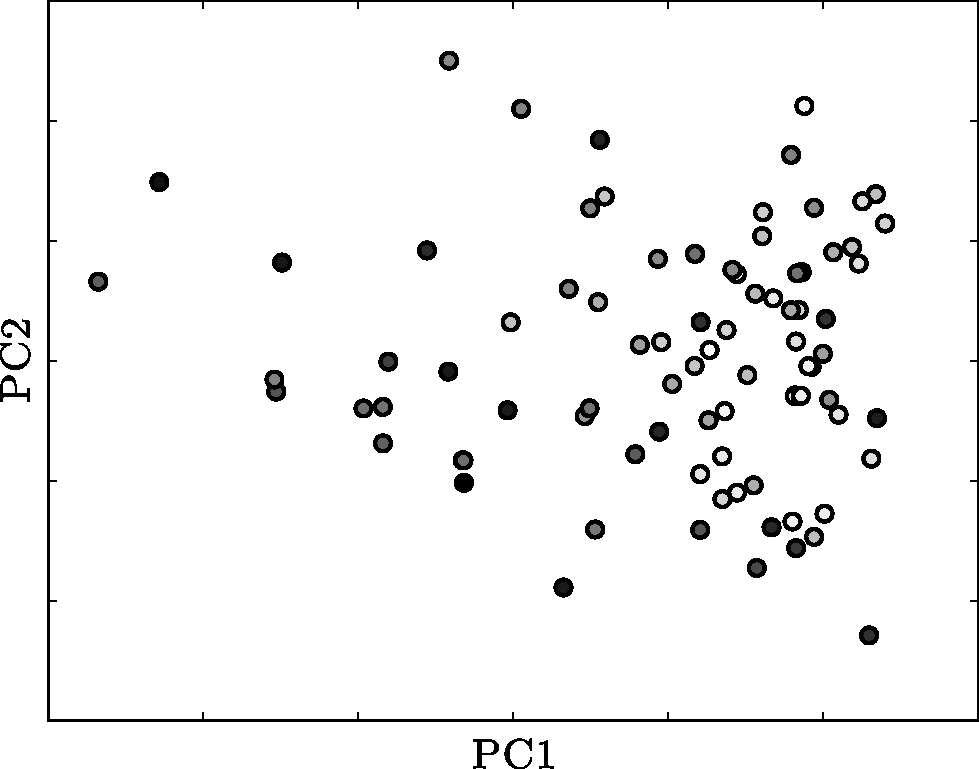
\includegraphics[width=0.5\columnwidth]{img/pca/pca-ace-fof1}\\
\vspace*{0.8cm}
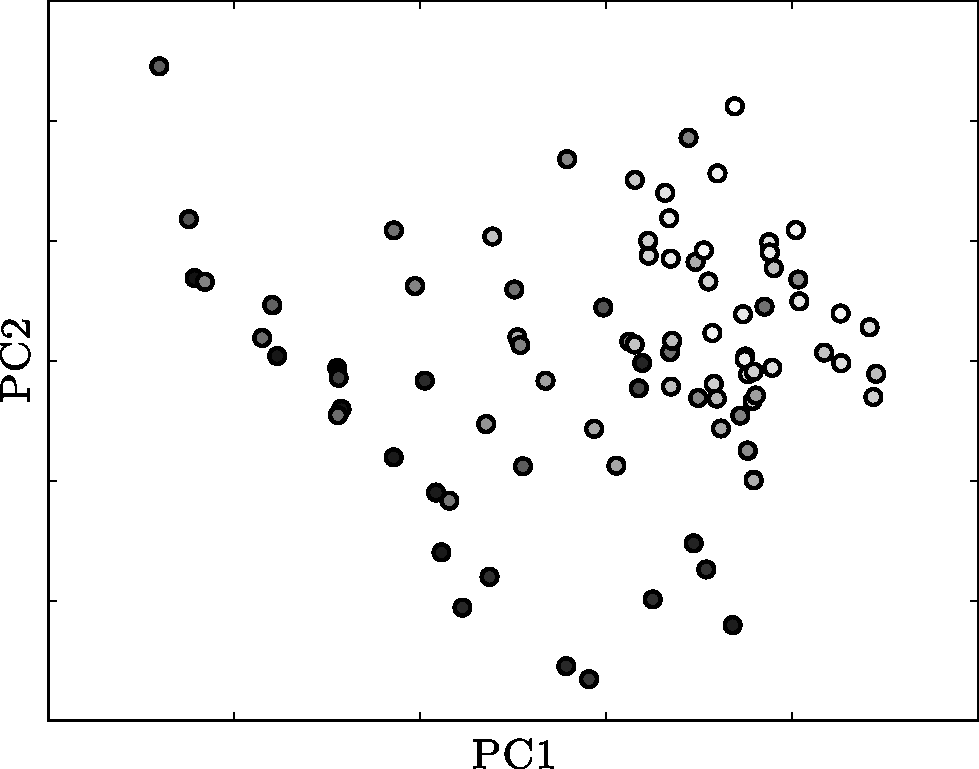
\includegraphics[width=0.5\columnwidth]{img/pca/pca-ace-fof2}\\
\vspace*{0.8cm}
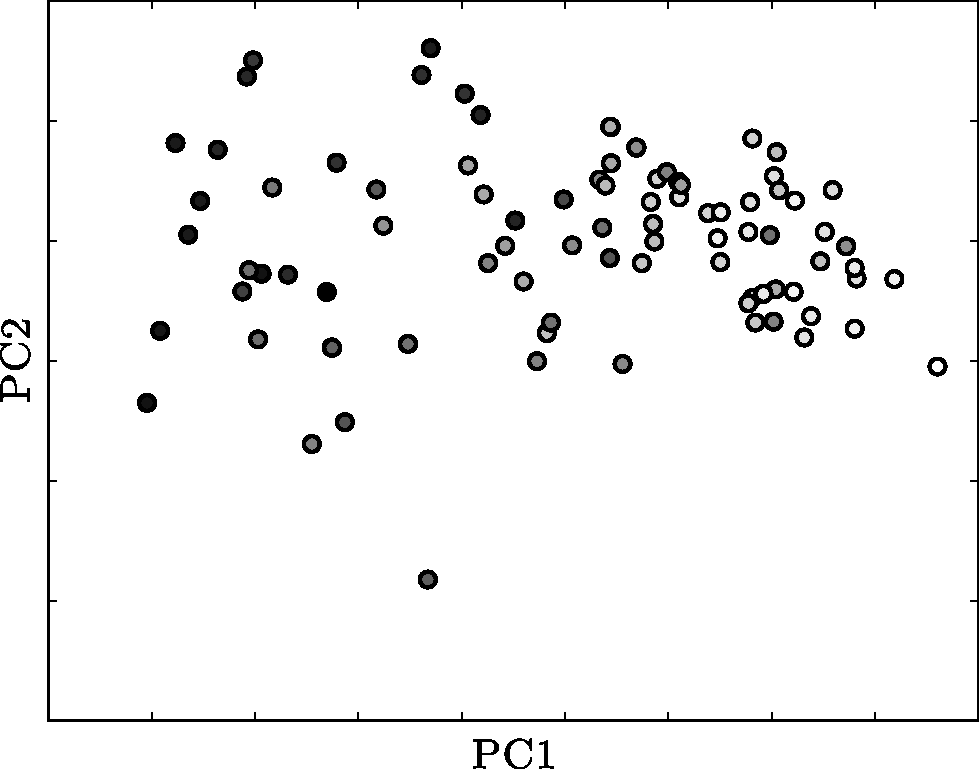
\includegraphics[width=0.5\columnwidth]{img/pca/pca-ace-fof3}\\
\medskip
\caption[PCA dei reservoir. GraphESN-FOF su ACE.]{Plot delle prime due componenti principali dello spazio degli stati dei reservoir nelle sotto-reti. Modello GraphESN-FOF applicato al task ACE.\\ 
In scuro gli input con valori target più alti.\\
Reservoir riportati: (\emph{alto}) sotto-rete 1; (\emph{centro}) sotto-rete 4; (\emph{basso}) sotto-rete 9.}
\label{fig:esperimenti:pca-ace-fof}
\end{figure}
%
\begin{figure}[p]
\centering
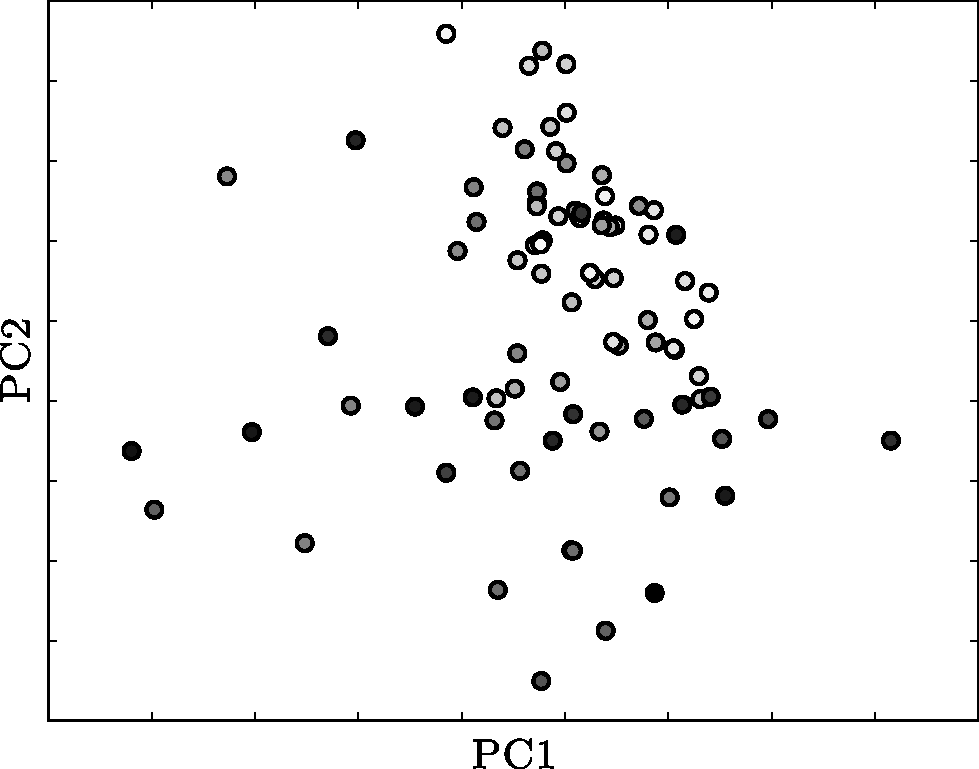
\includegraphics[width=0.5\columnwidth]{img/pca/pca-ace-nofof1}\\
\vspace*{0.8cm}
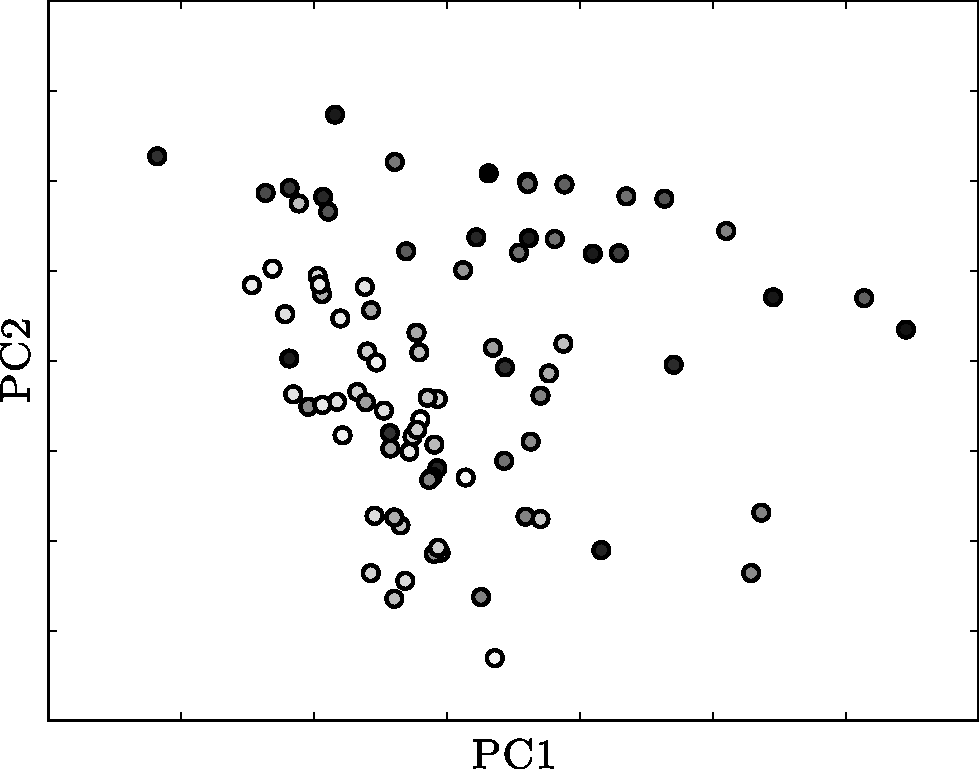
\includegraphics[width=0.5\columnwidth]{img/pca/pca-ace-nofof2}\\
\vspace*{0.8cm}
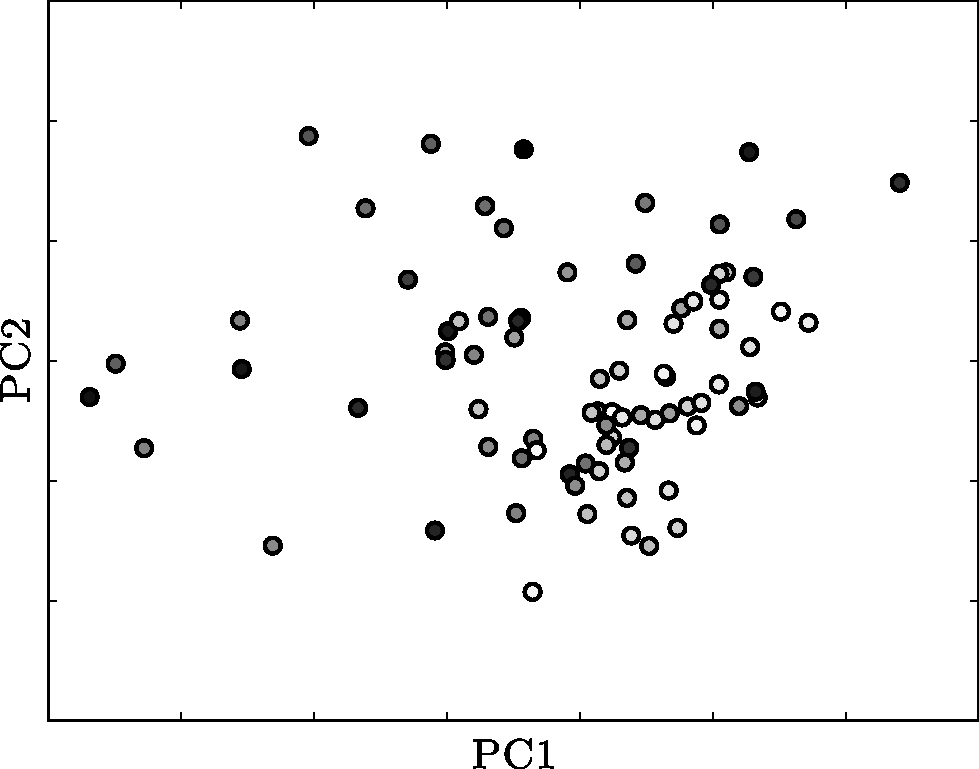
\includegraphics[width=0.5\columnwidth]{img/pca/pca-ace-nofof3}\\
\medskip
\caption[PCA dei reservoir. GraphESN-CF su ACE.]{Plot delle prime due componenti principali dello spazio degli stati dei reservoir nelle sotto-reti. Modello GraphESN-CF applicato al task ACE.\\ 
In scuro gli input con valori target più alti.\\
Reservoir riportati: (\emph{alto}) sotto-rete 1; (\emph{centro}) sotto-rete 5; (\emph{basso}) sotto-rete 9.}
\label{fig:esperimenti:pca-ace-nofof}
\end{figure}

L'efficacia dell'adozione di uno schema di output-feedback è inoltre confermata, secondo un approccio diverso, dall'analisi della capacità di fitting dei modelli. 
La figura~\ref{fig:esperimenti:confronto} mostra il confronto fra l'errore commesso, a parità di iperparametrizzazione ed al crescere della rete. Oltre ai tre proposti è stato in questo caso considerato un quarto modello, consistente in una GraphESN-FOF con connessioni di output-feedback che andassero unicamente verso i reservoir delle sotto-reti successive, e non anche verso il readout. 
Tenendo in considerazione il solo errore commesso sul training-set, ovvero la semplice capacità di fitting dei modelli, risulta evidente dal grafico come l'introduzione di informazione supervisionata attraverso gli output-feedback determini una accresciuta capacità di approssimazione da parte del modello.
\begin{figure}[tbp]
\centering
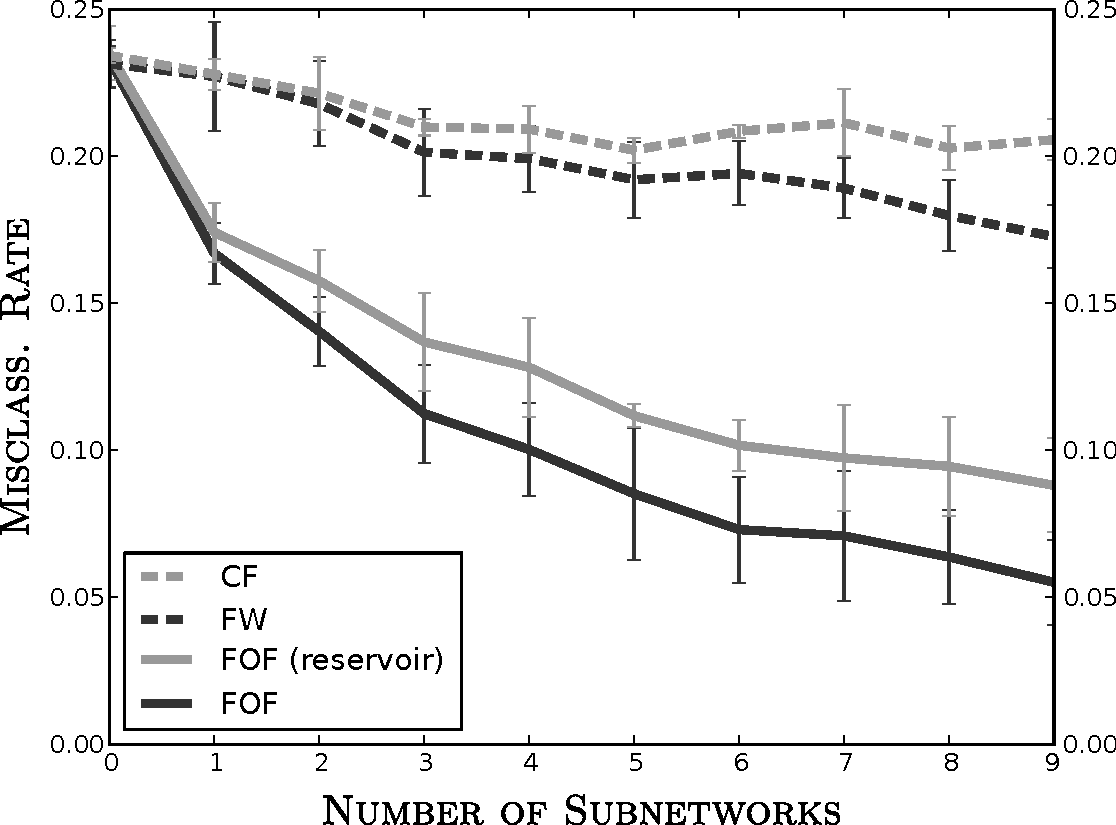
\includegraphics[width=0.7\columnwidth]{img/confronto-modelli-v2}
\medskip
\caption[Confronto fra i modelli: errore di training]{Confronto fra i modelli: errore di training (i.e.\ misclassification rate) e deviazione standard al crescere della rete. Task PTC-FM, $N_R = 100$.}
\label{fig:esperimenti:confronto}
\end{figure}


Dalle analisi supplementari risulta dunque come l'introduzione degli output-feedback rappresenti effettivamente una importante risorsa tesa a potenziare l'encoding delle reti, superando in parte i limiti legati all'uso di reservoir non adattivi. A fronte di questo, le osservazioni sia qualitative che quantitative sui risultati sperimentali suggeriscono l'impiego di forti meccanismi di regolarizzazione e di criteri di stop sofisticati, che impediscano alla rete di accrescere eccessivamente la propria complessità.

Sul piano pratico, gli esperimenti lasciano invece emergere un altro aspetto critico. Poiché per la natura del Reservoir Computing la dimensione del reservoir è estremamente importante ai fini del funzionamento della rete, è infatti necessario stabilire a priori quali siano le dimensioni dei reservoir delle sotto-reti. Nel farlo ci si trova di fronte ad una sorta di trade-off:
\begin{itemize}
\item Con $N_R$ troppo piccolo i reservoir delle sotto-reti perdono la capacità di espandere l'input su uno spazio degli stati ad alta dimensionalità, riducendo la capacità di apprendimento delle sotto-reti e della rete nel suo complesso. In questo scenario, inoltre, si rischia di perdere il vantaggio computazionale, pagando il prezzo di un numero molto alto di iterazioni necessarie alla costruzione della rete (si veda il paragrafo~\vref{sec:modelli:costo}). D'altra parte l'utilizzo di sotto-reservoir di piccole dimensioni offre l'opportunità di avere maggiore controllo sulla crescita della rete, che avverrà in maniera poco discontinua.
\item Con $N_R$ troppo grande si ottengono al contrario singole sotto-reti con una grande capacità di apprendimento che però più facilmente metteranno la rete nella condizione di incappare in situazioni di overfitting. L'aggiunta di una singola sotto-rete determina infatti in questo scenario un aumento elevato, e più difficilmente controllabile, della complessità del modello, rendendo complesso il compito di  apprendere dinamicamente una topologia che sia effettivamente adeguata al task affrontato.
\end{itemize}
Pur consentendo la determinazione automatica della topologia della rete, dunque, l'approccio costruttivo necessita di accorgimenti specifici che permettano di controllare la complessità della rete, attraverso esperienza empirica, criteri di stop sofisticati e l'adozione di meccanismi di regolarizzazione che possano evitare il verificarsi di situazioni di overfitting.












%%%%%%%%%%%%%%%%%%%%%%%%%%%%%%%%%%%%%%%%%%%%%%%%%%%%%%%%%%%%%%%%%%%%%%%%%%%%%%%
%%%%%%%%%%%%%%%%%%%%%%%%%%%%%%%%%%%%%%%%%%%%%%%%%%%%%%%%%%%%%%%%%%%%%%%%%%%%%%%


\begin{comment}

Misclassification-Rate

******************************* PTC FR *****************************************

*** Standard:   TR: 0.309 (stdev. 0.006)    TS: 0.323 (stdev. 0.014)
*** ZERO 50xX:  TR: 0.316 (stdev. 0.009)    TS: 0.327 (stdev. 0.019)
*** ZERO 30xX:  TR: 0.315 (stdev. 0.010)    TS: 0.328 (stdev. 0.018)
*** FW 50xX:    TR: 0.312 (stdev. 0.008)    TS: 0.329 (stdev. 0.010)
*** FW 30xX:    TR: 0.310 (stdev. 0.005)    TS: 0.328 (stdev. 0.004)
*** FOF 50xX:   TR: 0.299 (stdev. 0.007)    TS: 0.317 (stdev. 0.015)
*** FOF 30xX:   TR: 0.299 (stdev. 0.008)    TS: 0.321 (stdev. 0.013)

******************************* PTC FM *****************************************

*** Standard:   TR: 0.351 (stdev. 0.014)    TS: 0.393 (stdev. 0.042)
*** ZERO 50xX:  TR: 0.341 (stdev. 0.017)    TS: 0.372 (stdev. 0.042)
*** ZERO 30xX:  TR: 0.345 (stdev. 0.015)    TS: 0.368 (stdev. 0.044)
*** FW 50xX:    TR: 0.345 (stdev. 0.014)    TS: 0.364 (stdev. 0.044)
*** FW 30xX:    TR: 0.343 (stdev. 0.015)    TS: 0.367 (stdev. 0.038)
*** FOF 50xX:   TR: 0.344 (stdev. 0.017)    TS: 0.375 (stdev. 0.036)
*** FOF 30xX:   TR: 0.347 (stdev. 0.014)    TS: 0.372 (stdev. 0.035)

******************************* PTC MR *****************************************

*** Standard:   TR: 0.400 (stdev. 0.009)	TS: 0.433 (stdev. 0.036)
*** ZERO 50xX:  TR: 0.404 (stdev. 0.009)	TS: 0.421 (stdev. 0.021)
*** ZERO 30xX:  TR: 0.406 (stdev. 0.011)    TS: 0.419 (stdev. 0.019)
*** FW 50xX:    TR: 0.402 (stdev. 0.007)    TS: 0.416 (stdev. 0.017)
*** FW 30xX:    TR: 0.407 (stdev. 0.012)    TS: 0.426 (stdev. 0.021)
*** FOF 50xX:   TR: 0.388 (stdev. 0.017)	TS: 0.428 (stdev. 0.021)
*** FOF 30xX:   TR: 0.389 (stdev. 0.011)	TS: 0.426 (stdev. 0.016)

******************************* PTC MM *****************************************

*** Standard:   TR: 0.326 (stdev. 0.007)    TS: 0.329 (stdev. 0.033)
*** ZERO 50xX:  TR: 0.331 (stdev. 0.004)    TS: 0.350 (stdev. 0.024)
*** ZERO 30xX:  TR: 0.333 (stdev. 0.006)    TS: 0.342 (stdev. 0.023)
*** FW 50xX:    TR: 0.323 (stdev. 0.008)    TS: 0.346 (stdev. 0.032)
*** FW 30xX:    TR: 0.321 (stdev. 0.003)    TS: 0.354 (stdev. 0.027)
*** FOF 50xX:   TR: 0.311 (stdev. 0.012)    TS: 0.334 (stdev. 0.030)
*** FOF 30xX:   TR: 0.319 (stdev. 0.006)	TS: 0.346 (stdev. 0.023)



******************************* Mutag AB ***************************************

*** Standard:   TR: 0.203 (stdev. 0.015)    TS: 0.248 (stdev. 0.130)
*** ZERO 50xX:  TR: 0.150 (stdev. 0.014)	TS: 0.210 (stdev. 0.103) 
*** ZERO 30xX:  TR: 0.159 (stdev. 0.010)    TS: 0.204 (stdev. 0.102) 
*** FW 50xX:    TR: 0.138 (stdev. 0.009)    TS: 0.195 (stdev. 0.099)
*** FW 30xX:    TR: 0.141 (stdev. 0.009)    TS: 0.203 (stdev. 0.106)
*** FOF 50xX:   TR: 0.126 (stdev. 0.014)    TS: 0.207 (stdev. 0.053)
*** FOF 30xX:   TR: 0.131 (stdev. 0.007)    TS: 0.232 (stdev. 0.079)


******************************* Mutag AB+C *************************************

*** Standard:   TR: 0.163 (stdev. 0.019)    TS: 0.235 (stdev. 0.094)
*** ZERO 50xX:  TR: 0.162 (stdev. 0.022)    TS: 0.219 (stdev. 0.085)
*** ZERO 30xX:  TR: 0.174 (stdev. 0.025)    TS: 0.240 (stdev. 0.083)
*** FW 50xX:    TR: 0.163 (stdev. 0.016)    TS: 0.237 (stdev. 0.084)
*** FW 30xX:    TR: 0.161 (stdev. 0.018)    TS: 0.233 (stdev. 0.083)
*** FOF 50xX:   TR: 0.149 (stdev. 0.022)    TS: 0.240 (stdev. 0.075)
*** FOF 30xX:   TR: 0.159 (stdev. 0.027)    TS: 0.230 (stdev. 0.060)


******************************* Mutag AB+C+PS **********************************

*** Standard:   TR: 0.162 (stdev. 0.022)    TS: 0.197 (stdev. 0.066)
*** ZERO 50xX:  TR: 0.161 (stdev. 0.020)    TS: 0.206 (stdev. 0.085)
*** ZERO 30xX:  TR: 0.164 (stdev. 0.020)    TS: 0.203 (stdev. 0.082)
*** FW 50xX:    TR: 0.157 (stdev. 0.024)    TS: 0.207 (stdev. 0.083)
*** FW 30xX:    TR: 0.166 (stdev. 0.023)    TS: 0.194 (stdev. 0.072)
*** FOF 50xX:   TR: 0.158 (stdev. 0.021)    TS: 0.201 (stdev. 0.073)
*** FOF 30xX:   TR: 0.157 (stdev. 0.023)	TS: 0.200 (stdev. 0.080)

\end{comment}